\documentclass[11pt]{article}

\usepackage[margin=1.15in]{geometry}
\usepackage{amsmath,amssymb,amsthm}
\usepackage{booktabs}
\usepackage{array}
\usepackage{enumitem}
\usepackage{microtype}
\usepackage{xcolor}
\usepackage{hyperref}
\usepackage{natbib}
\usepackage{titlesec}
\usepackage{multirow}
\usepackage{graphicx}

%% Figures are in figures/ subdirectory as PDFs converted from SVGs

\hypersetup{colorlinks=true,linkcolor=black,citecolor=black,urlcolor=blue}
\titleformat{\section}{\large\bfseries}{\thesection}{1em}{}
\titleformat{\subsection}{\normalsize\bfseries}{\thesubsection}{1em}{}

%% Theorem environments
\newtheorem{definition}{Definition}[section]
\newtheorem{proposition}{Proposition}[section]
\newtheorem{theorem}{Theorem}[section]
\newtheorem{conjecture}{Conjecture}[section]
\theoremstyle{remark}
\newtheorem{observation}{Observation}[section]
\newtheorem{remark}{Remark}[section]
\newtheorem{example}{Example}[section]

%% Notation
\newcommand{\Gr}{\mathrm{Gr}}
\newcommand{\R}{\mathbb{R}}
\newcommand{\calM}{\mathcal{M}}
\newcommand{\calE}{\mathcal{E}}
\newcommand{\IIA}{\mathrm{IIA}}
\newcommand{\view}{\sigma}
\newcommand{\vO}{\mathcal{O}}
\newcommand{\vI}{\sim_{\sigma}}

\title{\textbf{What Is a Mechanism?}\\[0.3em]
\large A Five-Axis Ontology for Mechanistic Interpretability}
\author{Elliot Tower\\[0.1em]
\small \texttt{elliot@elliottower.ai}}
\date{}

\begin{document}
\maketitle

\begin{abstract}
Mechanistic interpretability has produced circuits, features, causal
subspaces, and activation-steered algorithms---each resting on an
implicit answer to a prior question: what kind of thing is a mechanism?
These are not terminological variants.  They differ in ontology, and
ontological differences propagate: what a mechanism \emph{is} determines
when two descriptions pick out the \emph{same} one, what \emph{evidence}
can warrant a claim, and what \emph{inferences} that claim licenses.
Many apparent disagreements in the literature are ontological
disagreements being conducted at the wrong level.

This paper introduces \emph{mechanistic views}: explicit background
accounts of what mechanisms are, how they are individuated, and what
evidence can support claims about them.  A view is a 5-tuple
$(O, {\sim}, E, F, T)$---an ontology, an identity criterion, an
evidential standard, a formalism, and an explanatory target.  We give
coherence conditions on this structure and show that incoherent views
produce unresolvable disagreements between evidence and identity:
disagreements that no additional experiment can settle, because each new
measurement either agrees with the declared identity criterion (adding
nothing) or conflicts with it (adding another contradiction).

The five components are not independent.  Ontology determines identity,
which determines formalism---a chain that explains why most coherence
violations are mismatches between the first three axes.  We present an
atlas of eight views currently operative in the literature, a five-axis
classification of 15 common interpretability methods by their implicit
view commitments, and four worked examples showing what each view claims
and what evidence each leaves open.

The framework is a diagnostic tool.  Making the view explicit lets
researchers state claims at the level their evidence supports, locate
disagreements at their source, and design experiments that discriminate
views rather than confirm them.
\end{abstract}

\tableofcontents
\newpage

%% ---------------------------------------------------------------
\section{Introduction}
%% ---------------------------------------------------------------

Mechanistic interpretability aims to explain what trained neural
networks are computing.  The field has made this aim concrete:
transformer circuits provide a component-level vocabulary for attention
heads and MLPs \citep{elhage2021}; induction heads account for a
mechanism involved in in-context learning \citep{olsson2022}; the
indirect object identification (IOI) circuit names the attention heads
involved in a specific syntactic task \citep{wang2022}; sparse
autoencoders recover interpretable directions from activation spaces
\citep{bricken2023,templeton2024}; causal abstraction methods test
whether high-level variables are realized in distributed representations
\citep{geiger2021,geiger2024}; and weight-space analyses recover
inter-layer communication channels and circuit structure from weight
matrices alone \citep{merullo2024,elhage2021}.

Yet the word \emph{mechanism} does not mean the same thing in all of
these cases.  In one paper a mechanism is a set of attention heads;
in another it is a functional role such as ``name mover''; in another
it is a causal subspace recovered by distributed alignment search; in
another it is a training-time transition.  These are not merely
terminological differences.  They carry different answers to five basic
questions:
\begin{enumerate}[leftmargin=*,label=(\arabic*)]
\item \textbf{Ontology}: what kind of entity counts as a mechanism?
\item \textbf{Identity}: when do two descriptions refer to the same mechanism?
\item \textbf{Evidence}: what measurements can warrant a claim about a mechanism?
\item \textbf{Formalism}: what mathematical language expresses the claim?
\item \textbf{Target}: what phenomenon is the mechanism supposed to explain?
\end{enumerate}
These questions are not new.  The philosophy of science has studied
mechanisms for decades: the Machamer-Darden-Craver (MDC) account defines
mechanisms as entities and activities organized to produce a phenomenon
\citep{machamer2000}; Glennan argues that mechanisms ground causal claims
\citep{glennan1996}; Craver develops mutual manipulability as the
criterion for constitutive relevance \citep{craver2007}; Bechtel and
Richardson study decomposition and localization as discovery strategies
\citep{bechtel1993}; and Illari and Williamson survey the diversity of
mechanism concepts across the sciences \citep{illari2012}.  What
interpretability adds is precision about the objects: neural network
mechanisms are computationally specified, fully inspectable, and amenable
to exact intervention.  What interpretability lacks is the conceptual
infrastructure that the philosophy of mechanisms provides.  This paper
bridges the gap.

Most published work answers these questions implicitly.  The answers are
recoverable from the methods used and the conclusions drawn, but they are
not stated---and because they are not stated, disagreements that are
fundamentally ontological are argued as disagreements about experimental
design.

\paragraph{Three motivating cases.}

\textbf{Underdetermination.}  Activation patching establishes that a
head is causally relevant to a behavior.  Does this establish a
mechanism?  Under the object view, perhaps yes.  Under the role view,
only if the functional role is independently specified and tested.
Under the subspace view, not unless the relevant variable is localized
to a specific causal subspace.  Under the structural view, not unless
the result is invariant under the relevant parameter symmetries.  A
single activation-patching result means different things under different
views, and the disagreement cannot be resolved by further patching
experiments alone---because all such experiments are equally consistent
with multiple views.

\textbf{Cross-model comparison.}  The claim that GPT-2 Small and
Pythia-160M implement the same induction head mechanism requires a
notion of mechanism identity that is cross-model.  Component indices are
trivially not cross-model.  Functional roles may be, if independently
specified.  Gauge-invariant subspace structure may be, if a canonical
transport map is defined.  Training-time trajectories may be, if the
dynamical basins correspond.  Which notion is operative determines
whether ``the same mechanism'' is meaningful across architectures---and
therefore whether cross-model generalization claims are well-formed.

\textbf{Safety-relevant inference.}  Safety work \citep{ngo2022} reasons
from ``circuit $X$ is present'' to ``the model has goal $Y$'' or ``the
model would behave $Z$ under distribution shift.''  These inferences require
different things depending on what a mechanism is.  Under an object view,
circuit presence is a fact about specific components in a specific model
on a specific distribution.  Under a structural view, a circuit present
as a gauge-invariant structure is robust to reparameterization.  Under
the instrumental view, a circuit label is warranted by behavioral
predictions.  The inference from circuit presence to safety-relevant
conclusion requires specifying which of these is operative.

\paragraph{Contributions.}
This paper makes three contributions:
\begin{enumerate}[leftmargin=*]
\item A formal definition of a \emph{mechanistic view} as a five-component
      structure $(O, {\sim}, E, F, T)$ with typed components and coherence
      conditions (\S\ref{sec:views}).
\item An atlas of eight views currently operative in the
      interpretability literature, with full axis assignments, evidence
      standards, discriminating experiments, and failure modes
      (\S\ref{sec:atlas}).
\item The determination chain---ontology implies identity implies
      formalism---with a five-axis methods mapping showing how common
      tools carry implicit view commitments
      (\S\ref{sec:chain}, \S\ref{sec:methods}).
\end{enumerate}
These are applied through four worked examples (\S\ref{sec:examples}),
five recurring decision points (\S\ref{sec:decisions}), and preliminary
cross-view promotion conditions (\S\ref{sec:implications}).

\paragraph{Relationship to Marr's levels.}
The most well-known framework for levels of analysis in computational
science is Marr's tri-level account \citep{marr1982}: a computational
level (what is computed and why), an algorithmic level (what
representation and process), and an implementational level (how the
algorithm is physically realized).  Marr's levels organize
\emph{explanatory targets}---they ask what a system does, how it does
it, and what substrate realizes the process.  The five axes here
organize \emph{ontological commitments}---they ask what kind of object
the mechanism is, when two are the same, and what evidence can support
the claim.  Marr's levels do not distinguish views: two researchers
at the same Marr level can hold different mechanistic views (object vs.\
subspace vs.\ structural).  The eight views are complementary to Marr's
hierarchy, not a refinement of it: both are needed, and neither
subsumes the other.


%% ---------------------------------------------------------------
\section{Mechanistic Views}\label{sec:views}
%% ---------------------------------------------------------------

\subsection{Formal Definition}

A mechanistic view is a background commitment that a researcher makes,
explicitly or implicitly, when they ask what a mechanism is.  We give
a formal definition, then unpack each component.

\begin{definition}[Mechanistic view]\label{def:view}
A \emph{mechanistic view} $\view$ is a tuple $(O, {\sim}, E, F, T)$
where:
\begin{enumerate}[leftmargin=*, label=(\roman*)]
\item $O$ is a set, the \textbf{ontology}, whose elements are the
      entities that count as mechanisms under $\view$.
\item ${\sim} \subseteq O \times O$ is an equivalence relation on $O$,
      the \textbf{identity criterion}: $x \sim y$ means descriptions $x$
      and $y$ refer to the same mechanism under $\view$.
\item $E$ is a set of \textbf{evidential standards}: pairs
      $(m, C)$ where $m$ is a measurement type and $C \subseteq
      2^O/{\sim}$ is the set of claims about equivalence classes of
      mechanisms that $m$ can in principle support.
\item $F$ is a \textbf{formalism}: a mathematical or representational
      language in which elements of $O$ can be expressed and $\sim$ can
      be computed.
\item $T$ is a \textbf{target}: a specification of the phenomena the
      view is designed to explain.
\end{enumerate}
\end{definition}

Several features of Definition~\ref{def:view} deserve comment.

The identity criterion $\sim$ is required to be an equivalence relation
(reflexive, symmetric, transitive).  This is not automatic: some
informal notions of mechanism identity in the literature are not
transitive.  For example, saying mechanisms $A$ and $B$ are ``related''
by shared components, and $B$ and $C$ are ``related'' by shared
function, does not imply $A$ and $C$ are the same mechanism.  Making
$\sim$ an equivalence relation forces precision.

The evidential standard $E$ is explicitly typed: each measurement type
$m$ is associated with the claims $C$ it can support.  This rules out
the common practice of using a measurement to support a claim that is
not in the range of that measurement.  Activation patching establishes
causal relevance of a component; it is not in the range of subspace
localization claims unless supplemented.

\begin{definition}[Coherence]\label{def:coherence}
A view $\view = (O, {\sim}, E, F, T)$ is \emph{coherent} if:
\begin{enumerate}[leftmargin=*, label=(\roman*)]
\item \textbf{Identity is grounded}: $\sim$ is definable using only
      the objects in $O$ and the language of $F$.  (A view whose
      identity criterion involves objects not in its own ontology is
      incoherent.)
\item \textbf{Evidence tracks identity}: for every measurement type
      $m \in E$, the claims $C(m)$ are expressible in terms of $\sim$-classes,
      not finer-grained distinctions.  (Evidence that distinguishes objects
      within a $\sim$-class is picking up on a different ontology than
      the one declared.)
\item \textbf{Formalism is expressive}: every element of $O$ has a
      representation in $F$, and $\sim$ is computable in $F$.
\end{enumerate}
\end{definition}

\begin{observation}[Incoherent views produce contradictory demands]\label{prop:incoherence}
Let $\view = (O, {\sim}, E, F, T)$ be a view that violates coherence
condition (ii): there exists a measurement type $m \in E$ and objects
$x, y \in O$ with $x \sim y$ but $m(x) \neq m(y)$.  Then there exist
mechanistic claims that are simultaneously required by $\sim$ to be true
(since $x$ and $y$ are the same mechanism) and required by $E$ to be
false (since $m$ distinguishes them).  No experiment can satisfy both
demands.  This is immediate from the definitions: the claim $\phi$ =
``$x$ and $y$ are the same mechanism'' is asserted by $\sim$ and refuted
by $m$, so the view entails $\phi \wedge \neg\phi$.
\end{observation}

A stronger consequence follows: incoherent views are not merely
contradictory in principle but produce systematic evidential
underdetermination in practice.

\begin{observation}[Incoherent views produce systematic underdetermination]\label{prop:underdet}
Let $\view = (O, {\sim}, E, F, T)$ violate coherence condition (ii),
so there exist $x \sim y$ in $O$ with measurement $m \in E$ such that
$m(x) \neq m(y)$.  Then for every finite evidence set
$\{m_1, \ldots, m_k\} \subseteq E$ that includes $m$, there exist
mechanism hypotheses $H_1$ and $H_2$ such that: (a)~$H_1$ and $H_2$
are identical under $\sim$ (same mechanism), (b)~$H_1$ and $H_2$ are
distinguishable by the evidence set, and (c)~no additional evidence
from $E$ can resolve whether the difference is real or an artifact
of the mismatch.  This follows by taking $H_1 = H_2 = [x]_\sim =
[y]_\sim$ and observing that any further measurement $m' \in E$ either
agrees with $\sim$ (offering no information about the $m$-discrepancy)
or disagrees (introducing its own underdetermination).
\end{observation}

Proposition~\ref{prop:underdet} is the practical payoff: incoherent
views do not merely produce logical contradictions---they produce
\emph{unresolvable} disagreements between evidence and identity, where
each new measurement either agrees with the identity criterion (offering
no information about the discrepancy) or disagrees (adding another
unresolved conflict).  This is the formal version of the empirical
observation that debates between, say, activation-patching advocates and
DAS advocates cannot be settled by more of the same evidence when the
participants hold different implicit views.

Propositions~\ref{prop:incoherence} and~\ref{prop:underdet} are useful
diagnostically.  A common pattern in interpretability is to declare that
mechanisms are gauge-invariant structures (structural view ontology)
but then to use activation-patching results as evidence of mechanism
presence without checking gauge invariance.  If the patching result
changes under a reparameterization that preserves computation, it is
distinguishing objects that the structural view says are identical---and
by Proposition~\ref{prop:underdet}, no amount of additional
activation-patching evidence can resolve this mismatch.

\subsection{The Five Axes}\label{sec:axes}

We organize the components of Definition~\ref{def:view} into five named
axes.  The axes are not independent: as coherence requires, choices on
one axis constrain the others.

\paragraph{Ontology ($O$).}
What kind of entity counts as a mechanism \citep{quine1948}?
Options include: concrete
model components (heads, neurons, MLP sublayers, SAE dictionary
elements), functional roles (descriptions of what a component does
independently of which component does it), causal subspaces (linear or
nonlinear submanifolds of the residual stream that mediate a causal
variable), gauge-invariant structures (equivalence classes of weight
configurations under symmetries that preserve the computation),
temporally extended processes (formation pathways or execution
trajectories), points in a stratified mechanism space, measurement
perspectives, and predictive models.

\paragraph{Identity ($\sim$).}
When do two mechanism descriptions denote the same mechanism?  Options
include: component overlap ($x \sim y$ iff they name the same set of
heads or neurons), role equivalence ($x \sim y$ iff they specify the
same functional input--output mapping), subspace proximity ($x \sim y$
iff the principal angles between the causal subspaces are all below a
threshold $\theta$, i.e.\ geodesic distance on $\Gr(k,d)$ is small),
gauge-orbit membership ($x \sim y$ iff there exists a computation-preserving
symmetry $g$ with $g \cdot x = y$), and dynamical-basin membership
($x \sim y$ iff the formation trajectories converge to the same
attractor).

\paragraph{Evidence ($E$).}
What measurements can support what claims?  Key distinctions: activation
patching establishes causal relevance of components under a fixed
distribution; DAS/IIA with linear alignment constraints measures causal
subspace identity; weight composition scores measure structural
information flow independent of any input distribution; checkpoint
analysis establishes formation dynamics; multi-method robustness tests
perspectival convergence.  The formal epistemology of evidence
accumulation \citep{earman1992,howson1989} suggests that independent
evidence converges faster than correlated evidence---a principle that
grounds the triangulation requirement in the perspectival view.

\paragraph{Formalism ($F$).}
What representational language is appropriate?  Directed graphs (circuits);
functional decompositions (roles); Grassmannian geometry $\Gr(k,d)$
(subspaces); fiber bundles and gauge groups (structural view); dynamical
systems and phase portraits (process view); Whitney stratifications
(stratified view); measurement algebras (perspectival view).

\paragraph{Target ($T$).}
What is the mechanism supposed to explain?  A specific behavioral output
on a specific distribution; a functional class across models; a
representational variable across inputs; a computation class across
parameterizations; a formation event; a resolution-relative phenomenon;
or a behavioral prediction.

%% ---------------------------------------------------------------
\section{An Atlas of Views}\label{sec:atlas}
%% ---------------------------------------------------------------

We identify eight views currently operative in the literature.  Table~\ref{tab:atlas}
gives the full axis assignments; Figure~\ref{fig:axes} shows how the five axes organize
the eight views.  The views are not mutually exclusive:
a single paper may use several, and convergence across views constitutes
stronger evidence than any single view.  The point is to distinguish
them so that each view's commitments and limitations can be assessed
independently.

\begin{table}[ht]
\centering
\small
\setlength{\tabcolsep}{4pt}
\begin{tabular}{p{0.10\linewidth}p{0.15\linewidth}p{0.15\linewidth}p{0.17\linewidth}p{0.15\linewidth}p{0.15\linewidth}}
\toprule
\textbf{View} & \textbf{Ontology ($O$)} & \textbf{Identity ($\sim$)}
  & \textbf{Evidence ($E$)} & \textbf{Formalism ($F$)} & \textbf{Target ($T$)} \\
\midrule
Object
  & Concrete part: head, neuron, feature
  & Component overlap
  & Ablation, activation patching
  & Directed graph
  & Specific behavior \\[3pt]
Role
  & Functional role in computation
  & Role equivalence (same I/O mapping)
  & Role-specific causal tests, cross-model
  & Functional decomposition
  & Functional class \\[3pt]
Subspace
  & Causal subspace of residual stream
  & Same projector; $d_{\Gr} < \theta$
  & DAS/IIA (linear), subspace stability
  & $\Gr(k,d)$
  & Representational variable \\[3pt]
Structural
  & Gauge-invariant relational structure
  & Gauge-orbit membership
  & Holonomy, comp. scores, reparameterization
  & Fiber bundle quotient
  & Computation class \\[3pt]
Process
  & Formation trajectory or execution regime
  & Same trajectory type or dynamical basin
  & Training checkpoints, formation knockouts
  & Dynamical system
  & Mechanism origin \\[3pt]
Stratified
  & Point in stratified mechanism space
  & Same stratum + local equivalence
  & Dimensionality tests, localization diagnostics
  & Whitney stratification
  & Resolution-relative phenomenon \\[3pt]
Perspectival
  & Projection of mechanism onto context
  & Cross-method coherence
  & Multi-method robustness
  & Measurement algebra
  & Method-relative observation \\[3pt]
Instrumental
  & Useful predictive or interventional model
  & Predictive equivalence
  & Forecast accuracy, intervention utility
  & Model theory
  & Behavioral prediction \\
\bottomrule
\end{tabular}
\caption{The eight mechanistic views with full axis assignments.}
\label{tab:atlas}
\end{table}


\begin{figure}[t]
\centering
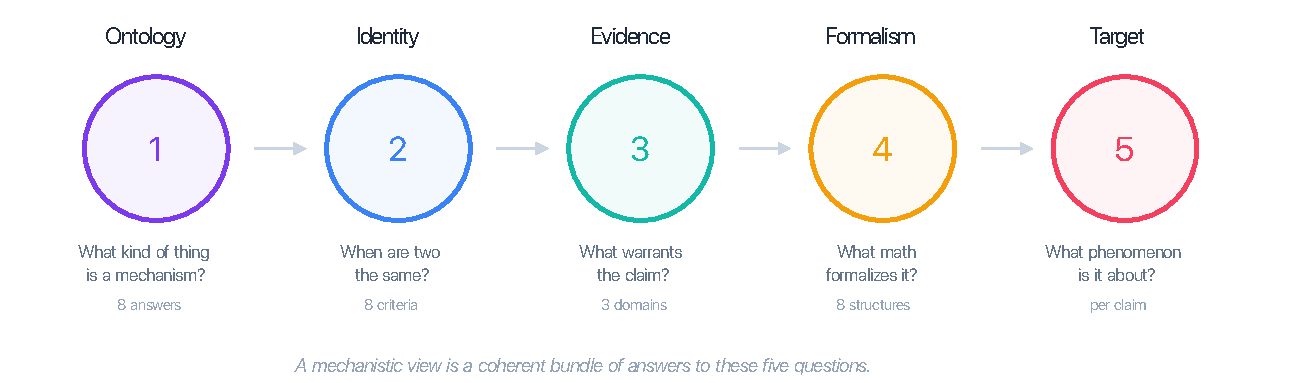
\includegraphics[width=\textwidth]{figures/five-axes-pipeline.pdf}
\caption{The five axes of a mechanistic view correspond to the five components
  of Definition~\ref{def:view}: $(O, {\sim}, E, F, T)$.  A mechanistic view is
  a coherent bundle of answers to these five questions.}
\label{fig:axes}
\end{figure}

\subsection{Object View}

The object view treats mechanisms as concrete model components: specific
attention heads, neurons, MLP sublayers, or sparse autoencoder dictionary
elements.  It is the implicit view in circuit diagrams.  The IOI circuit
as reported by \citet{wang2022}---26 attention heads organized into
functional groups---is an object-level description: the claim is about
those specific computational units.

\paragraph{Identity.}
Two circuit descriptions refer to the same mechanism iff they name the
same components.  This is precise within a model but trivially fails
cross-model: a head in GPT-2 Small is not an object in Pythia-160M.

\paragraph{Evidence.}
Ablation and activation patching are the natural evidence types.  Removing
a component's activation and observing behavioral degradation establishes
causal necessity; replacing it with a counterfactual activation establishes
causal sufficiency relative to that counterfactual.  The method is
strongest when the component set is stable across prompt distributions
and the ablation effect is large and specific.

\paragraph{Failure modes.}
\emph{Role inflation}: a component is identified by patching, then labeled
with a role (``name mover,'' ``induction head'') that implies richer
mechanistic content than the object-level evidence supports.  The component
identity is established; the role is a hypothesis.  \emph{Distribution
sensitivity}: the circuit identified by patching on one distribution may
differ substantially on another, meaning the claimed object-level mechanism
is distribution-relative.

\paragraph{Discriminating experiment.}
To test whether the object view is appropriate: ablate the identified
component set and test whether behavioral degradation is (a)~specific to
the behavior the mechanism is supposed to implement and (b)~stable across
prompt distributions.  If (b) fails, the object-level description is
distribution-relative and a role or subspace description may be more
appropriate.

\subsection{Role View}

The role view treats mechanisms as functional roles that can be realized
by different components---the role is a universal that can be multiply
instantiated \citep{lewis1986}.  ``Name mover'' is a role: it describes
what a component does (copy a name token to the output position), not
which head does it.  The role view explains why functionally equivalent
components across different models can be meaningfully compared.

\paragraph{Identity.}
Same functional input--output role, possibly in different components or
models.  Role identity requires a specification of the role that is
independent of the discovery procedure (i.e., not merely ``does what
this head does'') and tests that go beyond the ablation that revealed
the component.

\paragraph{Evidence.}
Role-specific predictions that are not entailed by mere causal relevance.
For a name-mover role claim: the weight-space signature of $W_{OV}$
should encode a copying operation; the head should perform this function
on novel prompts; a head in a different model with the same $W_{OV}$
signature should earn the same label.  The object-to-role slide is
a common source of overclaiming: establishing
that head 9.9 is causally necessary for IOI does not establish that it
is a name mover---the ablation evidence supports the object claim
(this component matters) but not the role claim (this component performs
a specific function) until the role is independently operationalized
and tested.

\paragraph{Failure modes.}
\emph{Role proliferation}: a new role label is coined for each component
discovered, re-describing the data without adding explanatory content.
\emph{Underdefined roles}: role labels are informal enough to be true of
any component, making them unfalsifiable.

\paragraph{Discriminating experiment.}
Take the role specification and apply it to a model in which the
original component has been ablated.  If the role is real, either another
component should take over (backup mechanism) or the behavior should
degrade in a specific role-consistent way.  If no such prediction is
confirmed, the role label has not been independently validated.

\subsection{Subspace View}

The subspace view treats mechanisms as low-dimensional causal subspaces
of the residual stream.  The key observation is that distributed
alignment search \citep{geiger2021,geiger2024} identifies not a component
but a rotation of the activation space: the causal variable is encoded
in a subspace that may span many components.  If alignment matrix $Q$
and its rotation $QR$ both achieve the same interchange intervention
accuracy (IIA), the relevant object is the subspace $\mathrm{span}(Q)$,
not the matrix $Q$.

\paragraph{Identity.}
Two subspace mechanisms are the same iff they project onto the same
subspace of $\mathbb{R}^d$: same projector $QQ^\top$, or equivalently
small geodesic distance on $\Gr(k,d)$.  This is basis-invariant and
can be meaningful cross-model when corresponding residual streams can
be aligned.

\paragraph{Evidence.}
The subspace view requires evidence that a specific subspace mediates a
causal variable, not merely that a search over subspaces finds one that
works.  Native subspace evidence includes: SVD or eigendecomposition of
weight matrices recovering the subspace without activation data;
Grassmannian distance between subspaces recovered by independent methods
(weight vs.\ activation); and subspace stability across prompt
distributions.  DAS and IIA are often cited as subspace evidence, but as
Table~\ref{tab:methods} shows, DAS is more precisely a Role-view method
with a borrowed subspace parameterization: it validates by intervention
success (role equivalence), not by Grassmannian distance.  DAS can
\emph{discover} a candidate subspace, but confirming that it is the
causally relevant subspace---rather than merely a subspace that permits
successful interchange---requires convergent evidence from weight-space
analysis.

\textbf{The Sutter constraint.}  \citet{sutter2025}\label{sutter}
showed that unrestricted nonlinear alignment maps achieve $100\%$ IIA
even on randomly initialized models, making DAS vacuous without
structural constraints on the alignment class.  Subspace-view claims
therefore require either linear alignment or alignment constrained to
respect the transport structure induced by the weight matrices.  Subject
to this constraint, subspace stability (eigenvalue gap between the causal
subspace and its complement) is the natural diagnostic.  This constraint
recurs throughout the atlas: it limits the evidential range of DAS
(Section~\ref{sec:methods}), appears in the diagnostic checklist
(Appendix~\ref{app:checklist}), and is the primary threat to subspace
claims in the worked examples.

\paragraph{Failure modes.}
\emph{SAE confusion}: sparse autoencoder features are dictionary elements
that minimize reconstruction loss; causal subspaces are directions that
mediate specific causal paths.  These are different objectives and can
disagree.  An SAE feature is a hypothesis about a one-dimensional
subspace mechanism, not a confirmed subspace claim.  \emph{Sutter vacuousness} (see above):
reporting high IIA without specifying the alignment class allows any
model to be assigned any causal structure.

\paragraph{Discriminating experiment.}
Verify that the identified subspace is stable: the subspace recovered
by DAS on a held-out distribution should have small geodesic distance
from the training-distribution subspace.  Also confirm that
an aligned basis-change (within the subspace) does not change the IIA,
while a rotation that takes vectors out of the subspace does reduce it.

\subsection{Structural View}

The structural view treats mechanisms as equivalence classes of
implementations under transformations that preserve the computation.
The relevant object is not a head index, a basis vector, or a specific
projection---it is the orbit of implementations related by the symmetry
group of the transformer's weight space.  Two weight configurations
that implement the same computation via different parameterizations are
the same mechanism under this view.

The formalism involves gauge orbits, parallel transport maps on the
Grassmannian, holonomy groups, and sheaf cohomology---the differential-geometric
toolkit of modern gauge theory \citep{nakahara2003}.

\paragraph{Identity.}
Gauge-orbit membership: $x \sim y$ iff there exists a computation-preserving
symmetry $g$ (such as a scale transformation, a rotation of a head's
query-key subspace paired with an inverse rotation of its output, or a
permutation of neurons) such that $g \cdot x = y$.  Holonomy fingerprints
provide a finer criterion: the holonomy group of the transport map
induced by a mechanism's weight matrices is an invariant that does not
change under gauge transformations.

\paragraph{Evidence.}
Gauge-invariant measurements: weight-space composition scores
$\|W_{O,u} W_{K,v}\|_F$ measure information flow capacity independently
of basis choice \citep{elhage2021,merullo2024}; holonomy measurements; and
reparameterization-stability tests (check that a result survives
computation-preserving rescalings of the weights).

\paragraph{Failure modes.}
\emph{False gauge invariance}: claiming structural equivalence without
verifying that the symmetry actually preserves the computation.
\emph{Architectural prior confound}: structural features that
discriminate trained from randomly initialized models may be detecting
architecturally privileged positions rather than learned structure.

\paragraph{Discriminating experiment.}
Apply a known computation-preserving symmetry (e.g., scale by $\lambda$,
counter-scale by $\lambda^{-1}$) to the weights of a component and
retest the activation-space evidence.  If the activation-space result
changes, the original result was not gauge-invariant and is not a
structural-view claim.

\subsection{Process View}

The process view treats mechanisms as temporally extended.  A mechanism
is not merely a final-checkpoint artifact but a formation process, an
execution trajectory, or a dynamical regime---what Darden calls
``reasoning about mechanisms in the making'' \citep{darden2006}.  This
view is natural for phenomena where the how of learning is itself
mechanistically relevant:
the induction head mechanism, for instance, forms via a phase transition
at a specific training step \citep{olsson2022}---this is process-level
structure that is not recoverable from the final checkpoint alone.

\paragraph{Identity.}
Same trajectory type or dynamical basin.  Two processes are the same
mechanism if they follow the same formation pathway, occupy the same
attractor, or exhibit the same phase-transition structure.  This notion
of identity is less developed than component or subspace identity, and
formalizing it is an open problem.

\paragraph{Evidence.}
Checkpoints, gradient flow, loss-curve structure, and formation knockouts.
A mechanism claim under the process view cannot be supported by
final-checkpoint analysis alone.  The induction head formation result
provides a clear example: the phase change at a specific training step
is visible in the composition score evolution, and this is process-level
evidence distinct from any claim about the final circuit \citep{olsson2022}.

\paragraph{Failure modes.}
\emph{Process--circuit conflation}: the final-checkpoint circuit and the
formation process are distinct objects; the circuit does not determine
the process.  Two models may arrive at identical final circuits via very
different training trajectories.  \emph{Training-detail overfitting}: a
process described precisely enough to be informative may be specific to
a particular optimizer, learning rate schedule, or dataset.

\paragraph{Discriminating experiment.}
Run the same architecture with different training hyperparameters (learning
rate, batch size, optimizer) and compare the formation dynamics.  If the
final circuit is similar but the formation trajectory differs, the
process-level claim is hyperparameter-sensitive and should be stated at
the appropriate level of generality.

\subsection{Stratified View}

The stratified view treats mechanism space as organized into strata:
point-localized objects, one-dimensional features, higher-dimensional
subspaces, nonlinear manifolds, and fully distributed structures.  Rather
than forcing a binary choice between localized and distributed, the
stratified view asks which stratum the evidence supports and whether the
appropriate description changes with measurement resolution.


\begin{figure}[t]
\centering
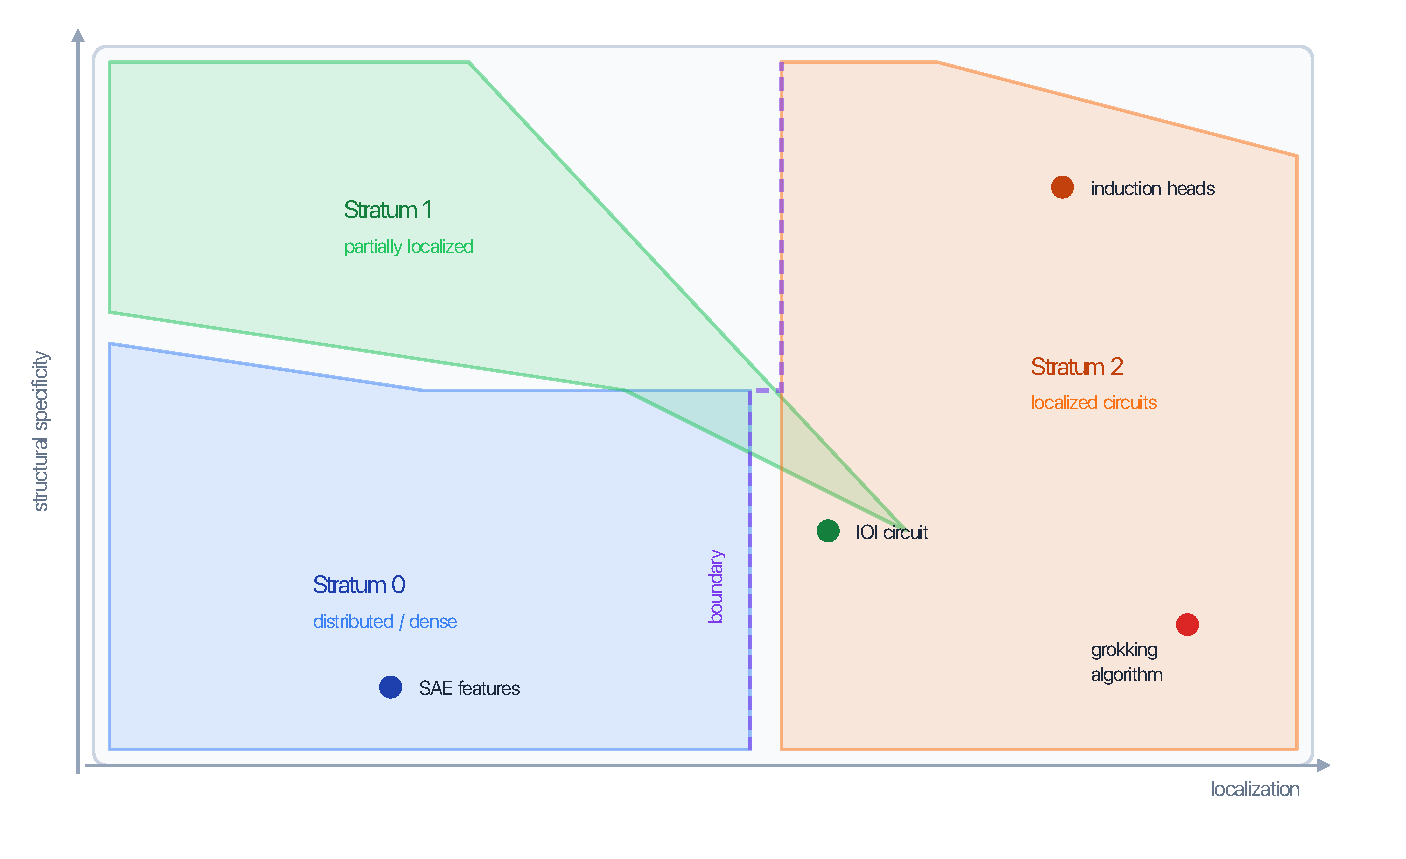
\includegraphics[width=\textwidth]{figures/strata-manifold.pdf}
\caption{Schematic of mechanism space as a stratified manifold.  Each stratum
  is a smoothly varying subset distinguished by the localization and structural
  specificity of the mechanism.  Boundaries between strata are lower-dimensional
  singular sets.  Empirical examples are placed roughly by the evidence reviewed
  in Section~\ref{sec:examples}; exact positions are schematic, not quantitative.}
\label{fig:strata}
\end{figure}

Figure~\ref{fig:strata} illustrates the key distinctions schematically.
The natural formalism is Whitney stratification \citep{whitney1965,golubitsky1973}:
a decomposition of mechanism space into smooth manifold strata that are
partially ordered by containment of their closures.  The stratified view
has a direct analogy in physics: the renormalization group (RG) describes
how the effective description of a system changes with measurement
resolution \citep{wilson1971,goldenfeld1992}.  RG fixed points correspond
to stable strata; relevant operators correspond to structure that survives
coarse-graining; universality classes correspond to mechanisms that appear
identical at a given resolution despite microscopic differences.  The
stratified view imports this resolution-dependence into interpretability.

A mechanism's stratum is determined
by its dimensionality, its localizability in specific components, and
the topology of its support in the residual stream.

\paragraph{Identity.}
Same stratum and same local equivalence class within the stratum.  Two
descriptions are the same mechanism if they name the same stratum and
agree on local structure within that stratum.

\paragraph{Evidence.}
Dimensionality tests (effective rank of the causal subspace),
localization diagnostics (is the mechanism's effect concentrated in a
small component set or distributed?), and stratum-transition tests
(does the apparent mechanism change stratum when the measurement
resolution changes?).

\paragraph{Failure modes.}
\emph{Stratum misidentification from method artifacts.}  A genuinely
distributed mechanism may appear localized to a single component if
the ablation method captures only the dominant direction.  Conversely,
a localized mechanism may appear distributed if the measurement method
has high background noise.  The stratified view does not resolve this
automatically---it provides the language to state it precisely.

\paragraph{Discriminating experiment.}
The stratified view predicts that measurement resolution affects the
apparent stratum.  Test this by comparing the effective dimensionality
of the causal subspace recovered by DAS at different hook points and
with different alignment constraints.  Consistent stratum across
resolutions supports a stratum assignment; stratum-change suggests
either a higher-stratum mechanism being partially recovered or a
measurement artifact.

\subsection{Perspectival View}

The perspectival view treats methods as revealing partial projections of
mechanisms rather than the mechanism in itself.  Disagreement between
methods is not automatically a failure; it may reveal the method-relative
structure of what is being measured.  This view is philosophically related
to Massimi's perspectival realism \citep{massimi2022}: the claim is not
that mechanisms are relative to methods (that would be instrumentalism),
but that scientific methods are partial perspectives on a
method-independent mechanistic structure.  The key distinction---between
perspectival \emph{evidence} (measurements are always from a vantage
point) and perspectival \emph{truth} (what's true depends on who measures
it)---maps directly onto the primary failure mode: conflating the
method-relativity of evidence with the claim that mechanisms are
themselves method-relative objects.

Identity is coherence across perspectives: two descriptions refer to the
same mechanism if they are mutually consistent and jointly interpretable
as projections of the same underlying structure.  Evidence is
multi-method robustness \citep{tower2026mechval}, formalized as
convergence across structural (weight), causal (activation/intervention),
and dynamic (training-time) evidence families.  The discriminating
experiment is cross-method consistency: test whether a patching-supported
claim is also supported by weight-space composition scores.  If not,
a third method adjudicates.

\subsection{Instrumental View}

The instrumental view treats mechanisms as useful predictive or
interventional models, warranted by forecast accuracy and intervention
utility regardless of whether they identify a real internal object.
Identity is predictive equivalence: two descriptions are the same
mechanism if they make the same predictions about all interventions and
behaviors.  This has the weakest ontological commitments and is therefore
the easiest to satisfy---but also the most limited.  The primary failure
mode is \emph{safety-relevant overreach}: claims that require strong
ontological conclusions (``the model is pursuing a goal'') cannot be
supported by predictive utility on the training distribution alone.
The discriminating experiment: test whether the mechanism label generates
novel predictions beyond the behavior used to identify it.

\subsection{The Determination Chain: Ontology Implies Identity Implies Formalism}\label{sec:chain}

The five axes are not independent.  In practice, the relationship is
mostly a chain of determination:
\[
\text{Ontology} \;\longrightarrow\; \text{Identity} \;\longrightarrow\; \text{Formalism}
\]
Choosing what kind of thing a mechanism \emph{is} determines when two
mechanisms are the \emph{same}, which in turn determines what
\emph{mathematical structure} can express the claim.  If mechanisms are
causal subspaces, identity is geodesic proximity on $\Gr(k,d)$, and the
formalism must include Grassmannian geometry.  If mechanisms are
gauge-invariant structures, identity is gauge-orbit membership, and the
formalism must include fiber bundles and holonomy groups.  The chain is
mostly one-to-one: each of the eight ontological commitments in the atlas
implies a specific identity criterion, which implies a specific ambient
formalism (Table~\ref{tab:atlas}).

Evidence and target are constrained by the ontology--identity pair but
not fully determined by it: a subspace claim can be supported by
activation-space evidence (DAS), weight-space evidence (SVD), or both,
and the target is chosen by the researcher.  The determination chain
therefore has two free parameters once the ontology is fixed.

This structure explains why the most common coherence violations involve
mismatches between the first three axes: using a subspace formalism
(Grassmannian distance) while holding an object ontology (component
overlap identity), or using an object evidence type (activation patching)
to support a structural claim (gauge-orbit identity).  The chain makes
these mismatches visible.

\subsection{View Families and Ontological Commitment}\label{sec:families}

The eight views group into three families and two singletons based on
their shared mathematical apparatus (Figure~\ref{fig:families}):

\begin{itemize}[leftmargin=*]
\item \textbf{Identity family} (Object, Role): mechanisms are identified
      by what they are (components) or what they do (functions).  Lowest
      mathematical overhead; most of the current literature operates here.
\item \textbf{Mathematical family} (Subspace, Structural): mechanisms
      live in geometric spaces and identity is defined by distances or
      orbits in those spaces.  Requires differential geometry.
\item \textbf{Process family} (Process, Stratified): mechanisms are
      temporally extended or resolution-dependent.  Requires dynamical
      systems theory or stratification theory.
\item \textbf{Methodological singleton} (Perspectival): no single
      method reveals the mechanism; identity requires cross-method
      coherence.
\item \textbf{Pragmatic singleton} (Instrumental): mechanisms are useful
      models; identity is predictive equivalence.
\end{itemize}

The views can be ordered by increasing ontological commitment---how much
they claim about the existence and nature of the mechanism independent of
any measurement procedure:
\[
\text{Instrumental} \;<\; \text{Perspectival} \;<\; \text{Object} \;<\;
\text{Role} \;<\; \text{Subspace} \;<\; \text{Structural} \;<\;
\text{Process} \;<\; \text{Stratified}
\]
Higher commitment views make stronger claims but require more evidence.
The instrumental view requires only predictive utility; the stratified
view requires evidence across multiple strata and measurement resolutions.
Most published interpretability work operates at the Object or Role level.
Moving to higher-commitment views---as this paper argues researchers
should consider---requires explicitly stating which view is operative and
supplying the corresponding evidence.

\begin{figure}[t]
\centering
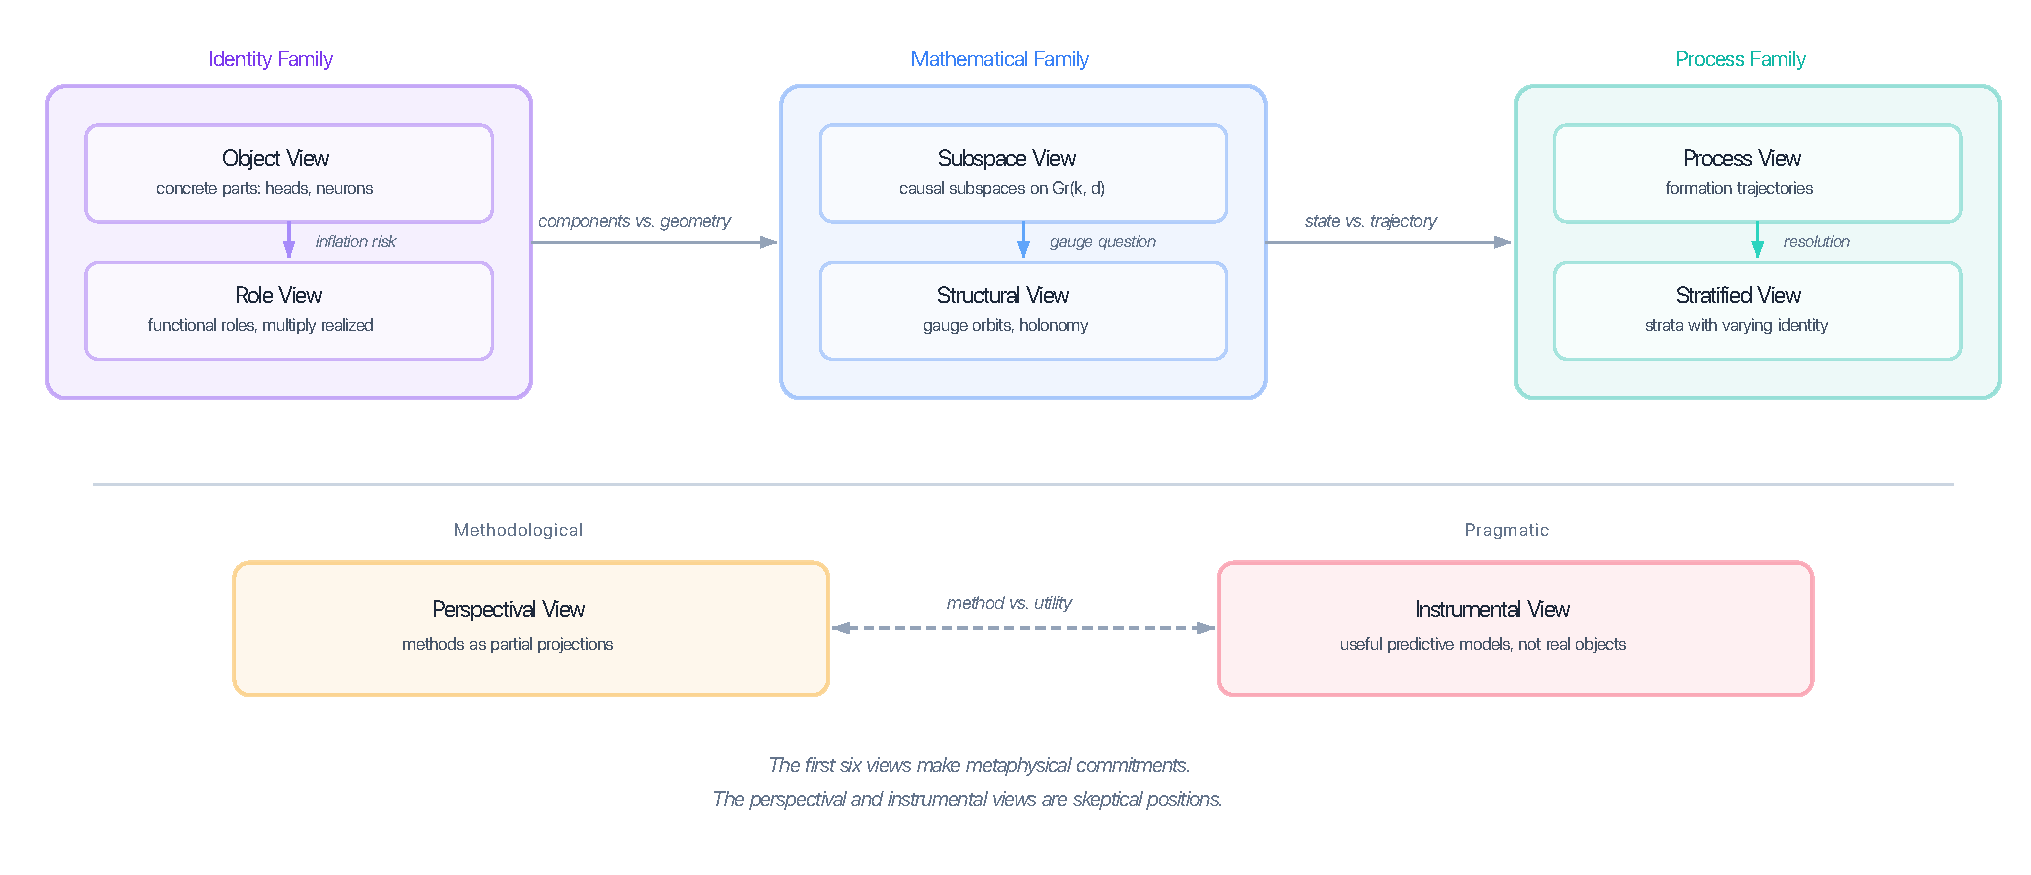
\includegraphics[width=\textwidth]{figures/eight-views-families.pdf}
\caption{The eight views grouped into three families (identity, mathematical,
  process) plus two singletons (methodological, pragmatic), ordered by
  increasing ontological commitment.  Within each family, the internal
  arrow marks the principal decision point between the two views.}
\label{fig:families}
\end{figure}

\begin{figure}[t]
\centering
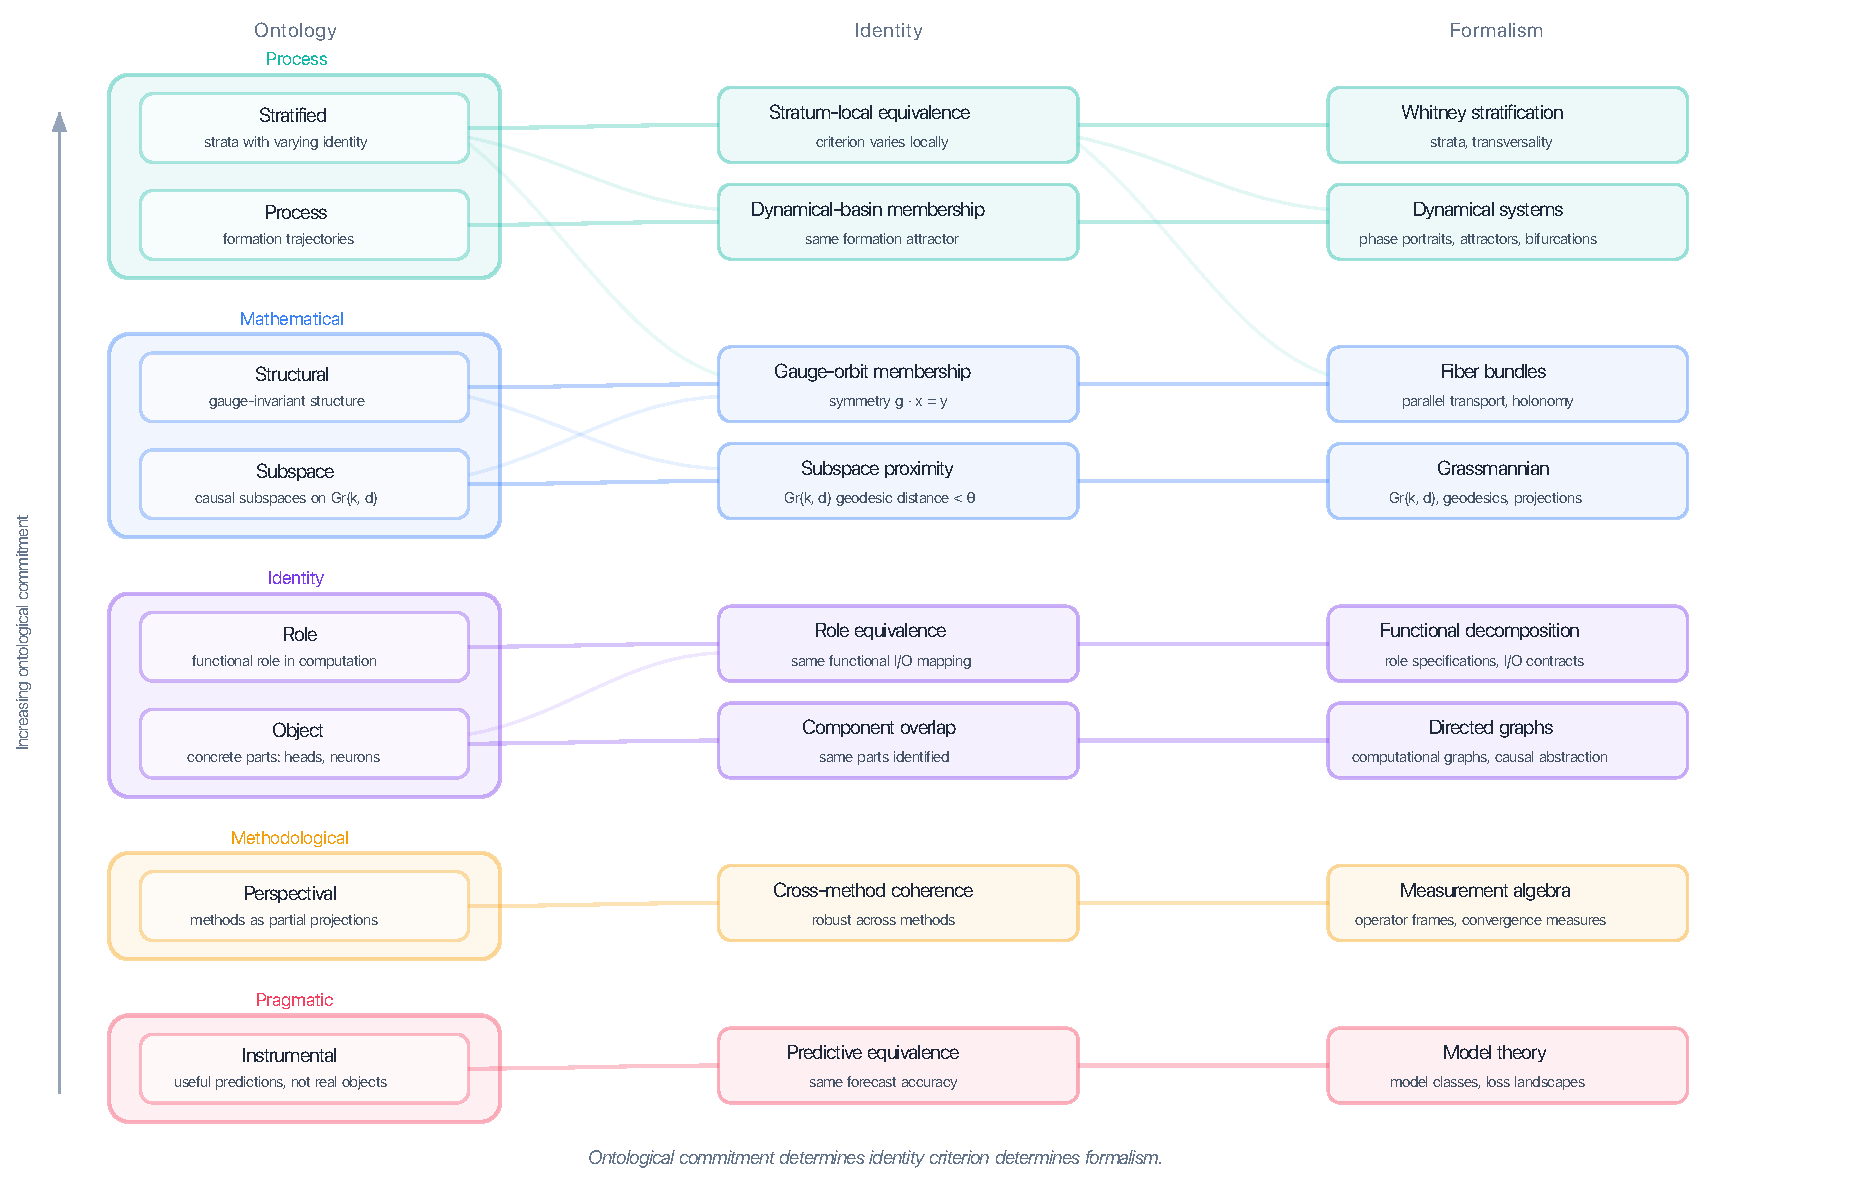
\includegraphics[width=\textwidth]{figures/ontology-identity-formalism.pdf}
\caption{The determination chain: ontology determines identity determines
  formalism.  Each view's ontological commitment (left) implies a specific
  identity criterion (center), which implies a natural mathematical formalism
  (right).  Primary connections are shown in bold; secondary cross-connections
  are shown faintly.  Increasing ontological commitment runs from bottom
  to top.}
\label{fig:determination}
\end{figure}

\subsection{Methods Mapping}\label{sec:methods}

Each commonly used interpretability method carries implicit commitments
across all five axes.  Table~\ref{tab:methods} makes these explicit.

\begin{table}[ht]
\centering
\small
\setlength{\tabcolsep}{3.5pt}
\begin{tabular}{p{0.15\linewidth}p{0.11\linewidth}p{0.14\linewidth}p{0.14\linewidth}p{0.16\linewidth}p{0.14\linewidth}}
\toprule
\textbf{Method} & \textbf{Ontology} & \textbf{Identity} & \textbf{Evidence} & \textbf{Formalism} & \textbf{Target} \\
\midrule
Activation patching & Object & Component overlap & Activations & Directed graph & Task circuit \\[2pt]
Path patching       & Object & Component overlap & Activations & Directed graph & Task circuit \\[2pt]
ACDC                & Object & Component overlap & Activations & Directed graph & Task circuit \\[2pt]
EAP                 & Object & Component overlap & Act.\ + Wt. & Directed graph & Task circuit \\[2pt]
Ablation            & Object & Component overlap & Activations & Directed graph & Importance \\[2pt]
DAS / IIA           & Role   & Role equivalence  & Activations & Subspace (borrowed) & Concept \\[2pt]
Causal scrubbing    & Role   & Role equivalence  & Activations & Causal graph & Alignment \\[2pt]
Linear probing      & Role   & Role equivalence  & Activations & Linear classifier & Detection \\[2pt]
SAE features        & Object & Component overlap & Activations & Dictionary & Feature catalog \\[2pt]
Logit / tuned lens  & Object & Component overlap & Activations & Linear proj. & Layer readout \\[2pt]
SVD of weights      & Subspace & Subspace prox. & Weights & $\Gr(k,d)$ & Decomposition \\[2pt]
Composition scores  & Structural & Gauge orbit  & Weights & Fiber bundle & Info-flow bound \\[2pt]
Factorization       & Subspace & Subspace prox. & Weights & $\Gr(k,d)$ & Decomposition \\[2pt]
Factor EAP          & Subspace & Subspace prox. & Wt.\ + Act. & $\Gr(k,d)$ + graph & Task circuit \\[2pt]
AGOP                & Process & Basin membership  & Dynamics & Dynamical sys. & Trajectory \\
\bottomrule
\end{tabular}
\caption{Five-axis classification of common interpretability methods.  Most
  methods are Object view with activation evidence.  DAS uses a subspace
  \emph{parameterization} but Role \emph{identity}: it validates by IIA
  success, not Grassmannian distance.  Factor EAP is the only method
  combining Subspace ontology with both weight and activation evidence.}
\label{tab:methods}
\end{table}

Several patterns are visible.  First, the field's default operating point
is Object ontology with activation evidence: activation patching, path
patching, ACDC, ablation, SAE features, and logit lens all sit here.
Second, DAS occupies an interesting intermediate position: it uses a
subspace parameterization (the alignment matrix $Q$ searches over
subspaces) but validates by interchange intervention accuracy, which is a
\emph{role}-level criterion---whether two representations can be swapped
without loss of function.  The subspace is the search space, not the
ontology.  Third, Factor EAP is the only method
that combines Subspace ontology with both evidence types: the factors
define the subspace decomposition (weight evidence), and the attribution
scores define which factors are active for a given task (activation
evidence).  Fourth, no widely-used method operates in the Stratified or
Perspectival views---these views generate research programs rather than
describing current practice.

%% ---------------------------------------------------------------
\section{Worked Examples}\label{sec:examples}
%% ---------------------------------------------------------------

Four extended examples show what the atlas does in practice: not just
describing views in the abstract, but showing how the same body of
evidence is read differently under different views and what each reading
implies for follow-up work.  The first three (IOI, induction heads, SAE
features) illustrate multi-view analysis of final-checkpoint phenomena.
The fourth (grokking) illustrates the process view, which cannot be
reduced to any final-checkpoint analysis.

\subsection{Indirect Object Identification}

\citet{wang2022} identify a circuit for indirect object identification
(IOI) in GPT-2 Small: 26 attention heads organized into functional
classes including S-inhibition heads, name movers, and
duplicate-token detection heads.

\paragraph{Object view.}
The mechanism is those 26 heads.  The evidence (activation and path
patching, mean ablation) establishes causal necessity and sufficiency
relative to the test distribution.  Object-level identity is precise
within GPT-2 Small and fails across architectures.

The object-level result is solid.  What it does not establish: (a) that
these heads perform a functional role that would be recognizable in
another model, (b) that the relevant causal variables are localized in
specific subspaces, (c) that the result is invariant under parameter
reparameterizations, or (d) how the circuit formed.  Claims (a)--(d)
require distinct evidence.

\paragraph{Role view.}
The four role classes (S-inhibition, name mover, duplicate-token
detection, and backup name mover) constitute a role-level description.
This is a hypothesis about what the heads do, not a confirmed role claim.
To confirm it, each role should be operationalized and tested
independently: name movers should copy tokens in novel syntactic
constructions; S-inhibition heads should suppress the subject in novel
contexts where the subject--object relationship is structurally varied.
Until these tests are run, the role labels describe the experimental
template more than the mechanism.

\paragraph{Subspace view.}
The subspace question is where the IO and S tokens, and the inhibitory
relationship between them, are represented in the residual stream.
DAS with linear alignment constraints would identify the causal
subspaces for each variable and test whether they can be independently
intervened on.  The 26-head object-level description does not resolve
this: two different subspace configurations could produce the same
patching results.

\paragraph{Structural view.}
The structural question is which aspects of the circuit are
gauge-invariant.  Path-patching results that survive
computation-preserving reparameterizations of the relevant head weights
establish structural facts; those that do not are basis-dependent
observations.  The holonomy of the circuit's transport map would provide
a structural fingerprint that is invariant across model instances.

\paragraph{What each view implies for next steps.}
Under the object view, the main open question is distribution
robustness: does the 26-head circuit generalize to other indirect
object constructions beyond the original template?  Under the role
view, it is role operationalization: what behavioral predictions do
the role labels generate beyond the original task?  Under the subspace
view, it is subspace identification and stability.  Under the structural
view, it is gauge-invariant characterization via the companion geometric
formalism.

\subsection{Induction Heads}

The induction head result \citep{olsson2022} is the strongest
mechanistic result in the current literature, precisely because multiple
views converge on the same object.

\paragraph{Object view.}
Induction heads are identified by activation patching.  Their distinctive
attention pattern---attending to the token immediately after the previous
occurrence of the current token---is established across a large family
of transformers.  Object-level identity is extended cross-model by
demonstrating the pattern holds across model sizes and architectures.

\paragraph{Role view.}
The induction pattern defines a functional role that is operationalized
(it can be tested on any sequence with a repeated token) and confirmed
across model families.  This is one of the few cases in the literature
where role identity is genuinely established rather than hypothesized.
The role specification is independent of the component: any head that
attends to $t_{j}$ from position $i$ when token $t_i = t_{j-1}$ is an
induction head, regardless of layer or position.

\paragraph{Process view.}
The formation dynamics are studied across training checkpoints.  A
phase transition is identified at a specific step in the loss curve,
and the composition score between the head and its prefix-matching
partner increases sharply at that step \citep{olsson2022}.  This is
process-level evidence---it concerns how the mechanism formed, not
what it is at the final checkpoint.  The formation process is argued
to be causally responsible for the in-context learning capacity of the
model, a claim that requires process evidence precisely because it is
about the training-time origin of a behavior.

\paragraph{What remains open.}
Under the stratified view: induction heads appear to be point-localized
objects, but whether the relevant causal variable is localized to a
one-dimensional subspace (object stratum) or spans a small-dimensional
subspace is not established.  Under the structural view: the holonomy
of the induction head transport map has not been characterized.  Under
the subspace view: the exact subspace of the residual stream encoding
the ``previous occurrence'' variable and the ``current token'' variable
has not been jointly identified via DAS.

The convergence across object, role, and process views is why the
induction head result can support relatively strong claims.  The gaps
in subspace and structural evidence are where further work would
strengthen or qualify those claims.

\subsection{Sparse Autoencoder Features}

Sparse autoencoder (SAE) features recovered from Claude-3 Sonnet
\citep{templeton2024} and smaller models \citep{bricken2023} are
semantically interpretable and partially causally validated via steering
experiments.  The status of SAE features as mechanisms is genuinely
contested, and the atlas provides precise vocabulary for the dispute.

\paragraph{Object view.}
Under the object view, each dictionary element is a potential mechanism:
a one-dimensional object in the activation space.  The evidence
(semantic interpretability, steering effects) supports a weak form of
causal relevance.  The object-level description is precise: the feature
is the specific dictionary vector learned by the SAE.

\paragraph{Subspace view.}
Each feature is a hypothesis about a one-dimensional causal subspace
mechanism.  The hypothesis is that the direction of the feature vector
corresponds to a direction in the residual stream that mediates a
specific causal variable.  The SAE training objective (sparse
reconstruction) does not guarantee this: the feature might be the
dominant activation direction without being the causally relevant one.
Confirmation requires linear DAS showing that the feature direction
specifically mediates the causal variable in question.

\paragraph{Perspectival view.}
SAE features are a measurement perspective on the activation space: the
perspective defined by the sparse coding objective.  This perspective
has specific invariances (insensitive to causal structure; sensitive to
geometric structure of activations) and specific blind spots (may
miss subspaces that are causally relevant but not reconstructively
prominent).  Under the perspectival view, the right question is not
``are SAE features mechanisms?'' but ``what does the SAE perspective
reveal that the weight-space perspective and the causal intervention
perspective would independently confirm?''  Convergence of all three
on the same direction would substantially strengthen the claim.

\paragraph{What each view implies for next steps.}
Under the object view: test causal necessity via ablation and compare
with the steering evidence.  Under the subspace view: run linear DAS
for the most interpretable features to test whether the feature
direction is the causal subspace direction for the relevant variable.
Under the perspectival view: compute weight-space composition scores
for the same features to identify which ones are also structurally
prominent, and compare with the causal evidence.

\subsection{Grokking: A Process-View Example}

Grokking---the phenomenon where a model suddenly generalizes to the test
set long after memorizing the training set---is the clearest case where
the process view is not optional.  A checkpoint analysis at any single
training step shows a model that has either memorized or generalized;
the mechanistically interesting phenomenon is the transition between
these regimes.

\paragraph{Process view.}
The mechanism is the formation trajectory itself: the transition from
memorization to generalization, the training step at which it occurs,
and the circuit-level changes that accompany it.  Identity under this
view is dynamical-basin membership: two models exhibit the same grokking
mechanism if they undergo structurally similar transitions (same
sequence of circuit formation events, same loss-curve topology) even if
the final circuits differ in detail.

\paragraph{Object view.}
An object-level analysis of the post-grokking checkpoint identifies the
circuit that implements the generalized computation.  This is a valid
object claim, but it misses the process-level structure entirely: it
cannot explain \emph{why} generalization happened, \emph{when} it
happened, or whether it would happen under different training conditions.

\paragraph{What each view implies.}
Under the process view: the key experiments are checkpoint sweeps,
formation knockouts (does ablating a component mid-training prevent the
transition?), and hyperparameter sensitivity (does the same transition
occur with different learning rates?).  Under the object view: the key
experiment is circuit identification at convergence.  The two views
answer different questions.  Neither subsumes the other, but claims about
the \emph{origin} of generalization require process evidence.

%% ---------------------------------------------------------------
\section{Five Decision Points}\label{sec:decisions}
%% ---------------------------------------------------------------

Five recurring forks in empirical interpretability work change in
meaning depending on which view is operative.  We examine what each
view implies for each fork and, where views make conflicting predictions,
what evidence would adjudicate.

\subsection{Localized vs.\ Distributed}

The question is whether a mechanism is implemented by a small, specific
set of components or spread across many.

Under the \emph{object view}, this is an empirical question: which
minimal component set is causally necessary and sufficient?  Under
the \emph{subspace view}, it is about the dimensionality and
localizability of the causal subspace: a low-rank subspace localized
in a small number of attention heads is one answer; a high-dimensional
subspace spanning many heads is another.  Under the \emph{stratified
view}, it is a question about which stratum the evidence supports.

The views come apart in practice.  Activation patching may identify a
small object-level component set as causally necessary, while DAS
identifies a high-dimensional subspace spanning many components.  These
need not be contradictory: the patching identifies the components whose
activation values lie in the relevant subspace; DAS characterizes the
subspace.  The stratified view provides the language to say that the
two results are compatible descriptions at different levels of
resolution.

\subsection{Object vs.\ Role}

The question is whether a mechanism claim is about a specific component
or about a functional role that component plays.  Under the \emph{object
view}, the claim is about the component; under the \emph{role view},
it is about the function.

The distinction matters for generalization.  An object claim does not
entail that any component in any other model is the same mechanism.  A
role claim does---if the role is operationalized and tested.  The slide
from object to role happens in one sentence in most papers (``head 9.9,
which we call a name mover, ...''): the object identity is
established, the role is named, and subsequent sentences treat the role
as established without independent validation.

\subsection{Single vs.\ Triangulated Evidence}

The question is whether a mechanistic claim requires evidence from a
single method or convergent evidence from multiple methods with
independent assumptions.

Under the \emph{object view} with activation patching, a single strong
patching result may be sufficient.  Under the \emph{subspace view},
weight-space and activation-space convergence strengthens the claim
(both should identify the same subspace if the view is correct).
Under the \emph{perspectival view}, single-method evidence is always
vulnerable to that method's confounds: triangulation is definitionally
required.

The case for triangulation is not merely a caution.  If a method $m$
can only support claims in its range $C(m)$, and the target claim is
not in $C(m)$, then no amount of evidence from $m$ can support the
claim---however strong that evidence is.

\subsection{Static vs.\ Process}

The question is whether the mechanism is a final-checkpoint artifact
or a formation process.  This is a clean view-level distinction with
a clean evidential consequence: process claims need process evidence;
checkpoint claims cannot support process conclusions.

This matters most for: (a) training-dynamics hypotheses (``the model
learned to do $X$ because ...''), (b) phase-transition-like generalization
patterns, and (c) claims about the origin of in-context learning
behaviors.  In all three cases, checkpoint evidence establishes what
the mechanism is at convergence but not how it came to be.

\subsection{Subspace vs.\ Structural}

The question is whether mechanism identity is determined by the subspace
a mechanism occupies or by the gauge-invariant structure of the
computation it performs.  A subspace claim is basis-invariant: the
subspace $\mathrm{span}(Q)$ is the same regardless of which orthonormal
basis of $Q$ is used.  But it is not symmetry-invariant: two subspace
mechanisms in the same gauge orbit (related by a computation-preserving
symmetry that rotates the subspace) would be the same mechanism under
the structural view but potentially different under the subspace view.

The structural view is more realist and harder to operationalize.  The
subspace view is more tractable and directly supported by current DAS
methodology.  For most practical questions in the field, the subspace
view is appropriate; the structural view becomes important when
comparing across parameterizations of the same architecture or when
making claims that should be invariant to training randomness.

\subsection{Behavioral vs.\ Mechanistic}

The question is whether a finding is about a model's \emph{behavioral
propensity} (how it tends to behave on a distribution) or about a
\emph{mechanism} (an internal structure that produces behavior).
\citet{steinhardt2026} argues that the field over-invests in capability
evaluation (can the model do~$X$?) and under-invests in propensity
evaluation (does the model typically do~$X$, and under what conditions?).

Under the \emph{instrumental view}, a behavioral finding---the model
reliably outputs~$Y$ given~$X$---is sufficient.  A propensity is what
you care about, and a mechanism is irrelevant.  Under the \emph{object
view}, a behavioral finding is a starting point: the question becomes
which components produce that behavior, and whether they are
necessary.  A capability finding (the model \emph{can} do~$X$) is
weaker than a propensity finding (the model \emph{typically does}~$X$)
because the former requires only that the relevant mechanism exists,
while the latter requires that it be routinely recruited.

The distinction matters most for safety.  A steering vector that
suppresses refusal behavior on a test distribution establishes an
instrumental capability---not a mechanistic understanding of
refusal~\citep{turner2024}.  Whether that vector \emph{is} the refusal
mechanism, or merely interferes with it, requires at least object-view
evidence (ablation of specific components) and ideally subspace-view
evidence (stability of the intervention direction across distributions).
The gap between instrumental evidence and the safety conclusions drawn
from it is the central evidence deficit identified by the open-problems
analysis in Appendix~\ref{app:openprobs}.


%% ---------------------------------------------------------------
\section{Practical Implications}\label{sec:implications}
%% ---------------------------------------------------------------

\paragraph{Stating the view is a publication norm.}
The primary practical implication of this paper is that mechanistic
interpretability claims should state the view under which they are made.
This is not bureaucratic overhead---it is a precision requirement of
the same kind as reporting which distribution patching was run on.
Appendix~\ref{app:checklist} provides a diagnostic checklist for
identifying coherence violations in published and in-progress work.
Object-level claims should be labeled as such, with the relevant
distribution specified.  Role claims should specify the role operationally
and report the independent tests.  Subspace claims should report the
identity criterion (same projector? geodesic distance below what
threshold?) and the subspace stability.  Structural claims should report
which symmetries were tested.  Process claims should report the
temporal evidence.

\paragraph{Evidence-claim matching.}
Each measurement type has a range: the set of claim types it can support.
A measurement whose range does not include the target claim type cannot
support that claim, regardless of how strong the measurement is.
Activation patching is not in the range of structural claims.
Single-method IIA without alignment constraint is not in the range of
any claim.  DAS with linear alignment is in the range of
one-dimensional subspace claims.  Stating the view makes these
range requirements explicit and checkable.

\paragraph{Independent convergence.}
\citet{williams2025} argue from philosophy of science that MI needs
philosophical foundations---for clarifying concepts, refining methods,
and navigating epistemic complexity.  Their three central examples
(decomposition identity, feature ontology, deception detection) map
directly onto view-level analyses in this paper: ``no single correct
decomposition'' corresponds to the object--subspace distinction
(Section~\ref{sec:axes}); ``vehicle vs.\ content'' corresponds to the
object--role split applied to features; and ``behavioral detection is
insufficient for deception'' corresponds to the instrumental view's
ceiling (Appendix~\ref{app:openprobs}).  The convergence from
independent starting points---philosophy of science vs.\ measurement
theory---strengthens both analyses and suggests that the underlying
structure is not an artifact of either framing.

\paragraph{Views as research programs.}
The object and role views primarily organize and classify existing
empirical practice.  The subspace, structural, and stratified views
generate positive research programs: each calls for methods, results,
and formalism that do not yet exist.  For the subspace view: systematic
DAS studies with stability tests across models and distributions.  For
the structural view: holonomy measurements, gauge-invariance checks,
and the development of the sheaf cohomology formalism.  For the
stratified view: dimensionality diagnostics and stratum-transition
tests.  The atlas is therefore not merely a taxonomy of current
practice; it is a map of what is missing.

%% ---------------------------------------------------------------
\section{Cross-View Promotion}\label{sec:promotion}
%% ---------------------------------------------------------------

\paragraph{Promotion conditions.}
A common question is: under what conditions can a result at one view be
promoted to a higher-commitment view?  The following are preliminary
promotion conditions:
\begin{itemize}[leftmargin=*]
\item \textbf{Object $\to$ Role.}  The component must be tested with an
      independently operationalized role specification on held-out
      constructions.  If the role predicts behavior beyond the original
      discovery distribution, the result can be stated as a role claim.
\item \textbf{Role $\to$ Subspace.}  The functional role must be shown to
      be mediated by a specific low-dimensional subspace (e.g., via linear
      DAS with the Sutter constraint), and this subspace must be stable
      across prompt distributions with small geodesic distance on $\Gr(k,d)$.
\item \textbf{Subspace $\to$ Structural.}  The subspace must survive
      computation-preserving symmetries of the weight space.  If the subspace
      recovered by DAS changes under a reparameterization that does not
      change the model's computation, the subspace claim is not structural.
      Holonomy measurements provide a gauge-invariant fingerprint.
\item \textbf{Any $\to$ Process.}  The static claim must be supplemented
      with training-dynamics evidence: checkpoint analysis showing when and
      how the mechanism formed, formation knockouts, or loss-curve structure.
      No amount of final-checkpoint evidence can substitute.
\end{itemize}
Each promotion requires new evidence of the kind specified by the target
view.  Evidence from the source view does not accumulate toward the
target view's standard---it answers a different question.  The chain is
not sequential: promotion can skip levels when the evidence supports it.
For example, an Object-level result can promote directly to Subspace if
linear DAS identifies a causal subspace spanning the relevant components,
without requiring an intermediate Role specification.  The subspace
evidence subsumes the object evidence (the components are where the
subspace has support) but does not require role-level mediation.

\paragraph{View selection: a practical heuristic.}
The framework is pluralist, but a researcher facing a concrete question
needs guidance on which view to adopt.  The following heuristic matches
the scope of the claim to the minimum view that can support it:
\begin{itemize}[leftmargin=*]
\item If the claim is about \emph{a specific model on a specific
      distribution}, the \textbf{Object view} is sufficient.
\item If the claim should \emph{generalize across models} (``Pythia and
      GPT-2 both have this mechanism''), at least the \textbf{Role view}
      is required---component indices are trivially not cross-model.
\item If the claim involves a \emph{distributed representation} not
      localized to a single component, the \textbf{Subspace view} is
      needed.
\item If the claim should \emph{survive reparameterization}
      (permutation, rescaling, rotation of weight matrices), the
      \textbf{Structural view} is needed.
\item If the claim is about \emph{how the mechanism formed} or why it
      appeared at a specific training step, the \textbf{Process view} is
      needed---no amount of checkpoint evidence can substitute.
\item If the mechanism's \emph{apparent type changes with measurement
      resolution}, the \textbf{Stratified view} is the appropriate
      language.
\end{itemize}
The heuristic is conservative: it recommends the lowest-commitment view
that matches the claim's scope.  Higher-commitment views are always
available but require correspondingly stronger evidence.

\paragraph{Connections to neighboring fields.}
The five-axis framework has natural translations into several disciplines
whose concepts it draws on.

\emph{Philosophy of science.}
The ontology axis corresponds to the central question of the new
mechanist literature: what counts as a mechanism
\citep{machamer2000,craver2007,illari2012,glennan1996}?  The identity
axis operationalizes the question that Lewis's possible-worlds
framework \citep{lewis1986} raises for functional kinds: under what
counterfactual conditions does a mechanism remain ``the same''?  The
evidence axis inherits the eliminativist structure of Earman's Bayesian
epistemology \citep{earman1992} and the domain-triangulation principle
of Howson and Urbach \citep{howson1989}: independent evidence types
eliminate distinct confounders.  Massimi's perspectival realism
\citep{massimi2022} maps directly onto the perspectival view, with
the important distinction that perspectival evidence does not entail
perspectival truth.

\emph{Physics.}
The structural view's gauge-invariance requirement is the direct
analogue of gauge symmetry in field theory: two weight configurations
related by a computation-preserving transformation are physically
the same mechanism, just as two vector potentials related by a gauge
transformation describe the same electromagnetic field
\citep{nakahara2003}.  The stratified view borrows the renormalization
group's central insight \citep{wilson1971,goldenfeld1992}: effective
descriptions change with measurement scale, and the interesting
objects are the fixed points (stable strata) and relevant operators
(structure that survives coarse-graining).  Universality classes
in physics correspond to mechanisms that appear identical at a given
resolution despite differing microscopically.

\emph{Mathematics.}
The formalism axis is not merely notational.  The choice of
mathematical structure constrains what can be stated precisely and
what can be proved.  Grassmannian geometry \citep{nakahara2003}
makes subspace proximity a metric statement; fiber bundles make
gauge invariance a theorem rather than a heuristic check; Whitney
stratification \citep{whitney1965,golubitsky1973} gives a rigorous
account of how mechanism identity changes across strata boundaries.
Each formalism carries proof obligations that the corresponding
informal claim does not.

\emph{Cognitive science and neuroscience.}
The localization--distribution spectrum (object view through stratified
view) mirrors the longstanding debate between localizationism and
distributed coding in systems neuroscience
\citep{bechtel1993}.  The double dissociation methodology in
neuropsychology---showing two functions can be selectively impaired
independently---is the nearest analogue to the necessity and
sufficiency tests used in the object view.  Marr's tri-level account
\citep{marr1982} organizes explanatory targets; the five axes here
organize ontological commitments.  Both are needed, and they are
complementary: two researchers at the same Marr level can hold different
mechanistic views.

%% ---------------------------------------------------------------
\section{Open Questions}\label{sec:open}
%% ---------------------------------------------------------------

Several questions are raised by the framework and not resolved:
\begin{enumerate}[leftmargin=*]
\item \emph{Process identity.}  The identity criterion for the process
      view (same dynamical basin or trajectory type) is underspecified
      relative to the object, subspace, and structural criteria.
      Formalizing process identity is an open problem.
\item \emph{Cross-view promotion.}  Under what conditions can an
      object-level result be promoted to a subspace-level or structural-level
      result?  Section~\ref{sec:promotion} gives preliminary conditions, but
      a systematic account of inter-view inference is missing.
\item \emph{Completeness of the atlas.}  The eight views are identified
      by reading the literature, not derived from the five axes.  Whether
      there are important views not represented---a Marr computational-level
      view \citep{marr1982}, a representational-content view, a
      population-level statistical view---is an open question.
\item \emph{Sufficiency of the five axes.}  The five axes may be too many
      or too few.  Evidence and formalism are tightly constrained by
      ontology and identity (the determination chain), raising the question
      of whether they are genuinely free axes or downstream consequences.
      Conversely, the framework omits a normative dimension---it diagnoses
      coherence but not adequacy for a given purpose.  Whether adequacy
      is a sixth axis or a meta-level concern about the framework is open.
\item \emph{View-independence of the framework.}  The framework itself
      is presented as view-neutral, but the formalization (equivalence
      relations, typed evidence) may privilege views whose identity criteria
      are crisp.  Whether the framework adequately represents views with
      inherently fuzzy identity (perspectival, process) is open.
\item \emph{Views and safety-relevant inference.}  Safety applications
      (monitoring, alignment auditing) require mechanistic claims that are
      robust to adversarial distribution shift.  What minimum view supports
      safety-relevant inference?  The object view is likely insufficient---a
      head identified as safety-relevant on one distribution may not
      generalize.  The structural or stratified views may be necessary, but
      their evidential demands are currently impractical at scale.
\item \emph{Implicit view commitments of existing programs.}  The
      monosemanticity program \citep{bricken2023,templeton2024} implicitly
      assumes that individual SAE dictionary elements are the right ontological
      unit (object view) with feature-level identity.  The causal abstraction
      program \citep{geiger2021,geiger2024} assumes role-level identity via
      interchange intervention.  Making these commitments explicit would
      clarify what each program can and cannot establish.
\end{enumerate}

%% ---------------------------------------------------------------
\section{Conclusion}
%% ---------------------------------------------------------------

Mechanistic interpretability is not only a search for circuits.  It is
a search for the right kind of object to call a mechanism.  The field
already uses multiple mechanistic views, typically implicitly, and making
those views explicit improves both the precision of claims and the
appropriateness of evidence.

The central contribution is definitional: a mechanistic view is a
five-component structure $(O, {\sim}, E, F, T)$, and every
mechanistic interpretability result assumes one, whether or not it is
stated.  Coherence between the components is not automatic: incoherent
views generate systematically unsatisfiable evidential demands
(Proposition~\ref{prop:incoherence}) and unresolvable underdetermination
(Proposition~\ref{prop:underdet}).  The determination chain---ontology
implies identity implies formalism---explains why most coherence
violations involve mismatches between these first three axes.

The atlas of eight views---object, role, subspace, structural, process,
stratified, perspectival, instrumental---covers the main options
currently in use.  Each view is appropriate for some questions and
inappropriate for others.  The paper is pluralist: the goal is not to
collapse this plurality into a master ontology but to make view choice
explicit, justifiable, and revisable.  Methods are discussed only in
their relation to views, not evaluated on their own technical merits.  The induction head result remains the canonical
illustration of what convergence across views looks like: object, role,
and process views all point to the same entity, which is why the result
supports claims that single-view results cannot.

%% ---------------------------------------------------------------
\bibliographystyle{plainnat}
\begin{thebibliography}{99}

\bibitem[Balesni et~al.(2024)]{apollo2024}
Mikita Balesni, Marius Hobbhahn, David Lindner, Alexander Meinke, Tomek
  Korbak, Joshua Clymer, Buck Shlegeris, Jeremy Scheurer, Charlotte Stix,
  et~al.
\newblock Towards evaluations-based safety cases for {AI} scheming.
\newblock arXiv:2411.03336, 2024.

\bibitem[Bechtel \& Richardson(1993)]{bechtel1993}
William Bechtel and Robert~C.\ Richardson.
\newblock \emph{Discovering Complexity: Decomposition and Localization as
  Strategies in Scientific Research}.
\newblock Princeton University Press, Princeton, NJ, 1993.

\bibitem[Bricken et~al.(2023)]{bricken2023}
Trenton Bricken, Adly Templeton, Joshua Batson, Brian Chen, Adam Jermyn,
  Tom Conerly, Nicholas L.\ Turner, Cem Anil, Carson Denison, Amanda Askell,
  Robert Lasenby, Yifan Wu, Shauna Kravec, Nicholas Schiefer, Tim Maxwell,
  Nicholas Joseph, Zac Hatfield-Dodds, Alex Tamkin, Karina Nguyen, Brayden
  McLean, Josiah E.\ Burke, Tristan Hume, Shan Carter, Tom Henighan, and
  Chris Olah.
\newblock Towards monosemanticity: Decomposing language models with dictionary
  learning.
\newblock \emph{Transformer Circuits Thread}, 2023.
\newblock \url{https://transformer-circuits.pub/2023/monosemanticity}.

\bibitem[Craver(2007)]{craver2007}
Carl F.\ Craver.
\newblock \emph{Explaining the Brain: Mechanisms and the Mosaic Unity of
  Neuroscience}.
\newblock Oxford University Press, Oxford, 2007.

\bibitem[Darden(2006)]{darden2006}
Lindley Darden.
\newblock \emph{Reasoning in Biological Discoveries: Essays on Mechanisms,
  Interfield Relations, and Anomaly Resolution}.
\newblock Cambridge University Press, Cambridge, 2006.

\bibitem[Earman(1992)]{earman1992}
John Earman.
\newblock \emph{Bayes or Bust? A Critical Examination of Bayesian Confirmation
  Theory}.
\newblock MIT Press, Cambridge, MA, 1992.

\bibitem[Elhage et~al.(2021)]{elhage2021}
Nelson Elhage, Neel Nanda, Catherine Olsson, Tom Henighan, Nicholas Joseph,
  Ben Mann, Amanda Askell, Yuntao Bai, Anna Chen, Tom Conerly, Nova DasSarma,
  Dawn Drain, Deep Ganguli, Zac Hatfield-Dodds, Danny Hernandez, Andy Jones,
  Jackson Kernion, Liane Lovitt, Kamal Ndousse, Dario Amodei, Tom Brown, Jack
  Clark, Jared Kaplan, Sam McCandlish, and Chris Olah.
\newblock A mathematical framework for transformer circuits.
\newblock \emph{Transformer Circuits Thread}, 2021.
\newblock \url{https://transformer-circuits.pub/2021/framework}.

\bibitem[Glennan(1996)]{glennan1996}
Stuart Glennan.
\newblock Mechanisms and the nature of causation.
\newblock \emph{Erkenntnis}, 44\penalty0 (1):\penalty0 49--71, 1996.

\bibitem[Geiger et~al.(2021)]{geiger2021}
Atticus Geiger, Hanson Lu, Thomas Icard, and Christopher Potts.
\newblock Causal abstractions of neural networks.
\newblock In \emph{Advances in Neural Information Processing Systems
  (NeurIPS)}, 2021.

\bibitem[Geiger et~al.(2024)]{geiger2024}
Atticus Geiger, Zhengxuan Wu, Christopher Potts, Thomas Icard, and Noah D.\
  Goodman.
\newblock Finding alignments between interpretable causal variables and
  distributed neural representations.
\newblock In \emph{Conference on Causal Learning and Reasoning (CLeaR)}, 2024.

\bibitem[Goldenfeld(1992)]{goldenfeld1992}
Nigel Goldenfeld.
\newblock \emph{Lectures on Phase Transitions and the Renormalization Group}.
\newblock Addison-Wesley, Reading, MA, 1992.

\bibitem[Golubitsky \& Guillemin(1973)]{golubitsky1973}
Martin Golubitsky and Victor Guillemin.
\newblock \emph{Stable Mappings and their Singularities}.
\newblock Springer-Verlag, New York, 1973.

\bibitem[Howson \& Urbach(1989)]{howson1989}
Colin Howson and Peter Urbach.
\newblock \emph{Scientific Reasoning: The Bayesian Approach}.
\newblock Open Court, La Salle, IL, 1989.

\bibitem[Illari \& Williamson(2012)]{illari2012}
Phyllis McKay Illari and Jon Williamson.
\newblock What is a mechanism? Thinking about mechanisms across the sciences.
\newblock \emph{European Journal for Philosophy of Science},
  2\penalty0 (1):\penalty0 119--135, 2012.

\bibitem[Machamer et~al.(2000)]{machamer2000}
Peter Machamer, Lindley Darden, and Carl F.\ Craver.
\newblock Thinking about mechanisms.
\newblock \emph{Philosophy of Science}, 67\penalty0 (1):\penalty0 1--25, 2000.

\bibitem[Lewis(1986)]{lewis1986}
David Lewis.
\newblock \emph{On the Plurality of Worlds}.
\newblock Blackwell, Oxford, 1986.

\bibitem[Marr(1982)]{marr1982}
David Marr.
\newblock \emph{Vision: A Computational Investigation into the Human
  Representation and Processing of Visual Information}.
\newblock W.\ H.\ Freeman, San Francisco, 1982.

\bibitem[Massimi(2022)]{massimi2022}
Michela Massimi.
\newblock \emph{Perspectival Realism}.
\newblock Oxford University Press, Oxford, 2022.

\bibitem[Nakahara(2003)]{nakahara2003}
Mikio Nakahara.
\newblock \emph{Geometry, Topology and Physics}.
\newblock Institute of Physics Publishing, Bristol, 2nd edition, 2003.

\bibitem[MIB(2025)]{mib2025}
Mechanistic Interpretability Benchmark.
\newblock Comprehensive evaluation for circuit discovery methods.
\newblock 2025.
\newblock \url{https://github.com/mechanistic-interpretability-benchmark/mib}.

\bibitem[Merullo et~al.(2024)]{merullo2024}
Jack Merullo, Carsten Eickhoff, and Ellie Pavlick.
\newblock Talking heads: Understanding inter-layer communication in transformer
  language models.
\newblock arXiv:2406.09519, 2024.

\bibitem[Nanda(2022)]{nanda2022open}
Neel Nanda.
\newblock 200 concrete open problems in mechanistic interpretability.
\newblock Blog post, 2022.
\newblock \url{https://www.neelnanda.io/mechanistic-interpretability/200-open-problems}.

\bibitem[Ngo et~al.(2022)]{ngo2022}
Richard Ngo, Lawrence Chan, and S\"oren Mindermann.
\newblock The alignment problem from a deep learning perspective.
\newblock arXiv:2209.00626, 2022.

\bibitem[Olsson et~al.(2022)]{olsson2022}
Catherine Olsson, Nelson Elhage, Neel Nanda, Nicholas Joseph, Nova DasSarma,
  Tom Henighan, Ben Mann, Amanda Askell, Yuntao Bai, Anna Chen, et~al.
\newblock In-context learning and induction heads.
\newblock \emph{Transformer Circuits Thread}, 2022.
\newblock \url{https://transformer-circuits.pub/2022/in-context-learning-and-induction-heads}.

\bibitem[Schmidt Futures(2026)]{schmidt2026}
Schmidt Futures.
\newblock Trustworthy AI research agenda.
\newblock Request for proposals, 2026.

\bibitem[Sharkey et~al.(2025)]{sharkey2025}
Lee Sharkey, Bilal Chughtai, Joshua Batson, Jack Lindsey, Jeff Wu, Lucius
  Bushnaq, Nicholas Goldowsky-Dill, Stefan Heimersheim, et~al.
\newblock Open problems in mechanistic interpretability.
\newblock arXiv:2501.16496, 2025.

\bibitem[Quine(1948)]{quine1948}
Willard Van~Orman Quine.
\newblock On what there is.
\newblock \emph{Review of Metaphysics}, 2\penalty0 (5):\penalty0 21--38, 1948.

\bibitem[Steinhardt(2026)]{steinhardt2026}
Jacob Steinhardt.
\newblock The case for evaluating model behaviors.
\newblock Alignment Forum, May 2026.

\bibitem[Sutter et~al.(2025)]{sutter2025}
Denis Sutter, Julian Minder, Thomas Hofmann, and Tiago Pimentel.
\newblock The non-linear representation dilemma: Is causal abstraction enough
  for mechanistic interpretability?
\newblock In \emph{Advances in Neural Information Processing Systems
  (NeurIPS)}, 2025.

\bibitem[Templeton et~al.(2024)]{templeton2024}
Adly Templeton et~al.
\newblock Scaling monosemanticity: Extracting interpretable features from
  {Claude 3 Sonnet}.
\newblock \emph{Anthropic Transformer Circuits Thread}, 2024.
\newblock \url{https://transformer-circuits.pub/2024/scaling-monosemanticity}.

\bibitem[Turner et~al.(2024)]{turner2024}
Alex Turner, Lisa Thiergart, Gavin Leech, David Udell, Juan~J.\ Vazquez,
  Ulisse Mini, and Monte MacDiarmid.
\newblock Activation addition: Steering language models without optimization.
\newblock arXiv:2308.10248, 2024.

\bibitem[Tower(2026)]{tower2026mechval}
Elliot Tower.
\newblock Mechanistic validity: A multi-discipline framework for evaluating
  mechanistic claims in neural networks.
\newblock Preprint, 2026.

\bibitem[Wang et~al.(2022)]{wang2022}
Kevin Wang, Alexandre Variengien, Arthur Conmy, Buck Shlegeris, and Jacob
  Steinhardt.
\newblock Interpretability in the wild: A circuit for indirect object
  identification in {GPT-2 Small}.
\newblock arXiv:2211.00593, 2022.

\bibitem[Williams et~al.(2025)]{williams2025}
Iwan Williams, Ninell Oldenburg, Ruchira Dhar, Joshua Hatherley, Constanza
  Fierro, Nina Rajcic, Sandrine~R.\ Schiller, Filippos Stamatiou, and Anders
  S{\o}gaard.
\newblock Mechanistic interpretability needs philosophy.
\newblock arXiv:2506.18852, 2025.

\bibitem[Whitney(1965)]{whitney1965}
Hassler Whitney.
\newblock Tangents to an analytic variety.
\newblock \emph{Annals of Mathematics}, 81\penalty0 (3):\penalty0 496--549, 1965.

\bibitem[Wilson(1971)]{wilson1971}
Kenneth G.\ Wilson.
\newblock Renormalization group and critical phenomena.\ {I}.\ Renormalization
  group and the {Kadanoff} scaling picture.
\newblock \emph{Physical Review B}, 4\penalty0 (9):\penalty0 3174--3183, 1971.

\bibitem[Woodward(2003)]{woodward2003}
James Woodward.
\newblock \emph{Making Things Happen: A Theory of Causal Explanation}.
\newblock Oxford University Press, Oxford, 2003.

\end{thebibliography}

\newpage
%% ---------------------------------------------------------------
\appendix
\section{Coherence Violations: A Diagnostic Checklist}\label{app:checklist}
%% ---------------------------------------------------------------

The following patterns indicate a coherence violation in the view
underlying a claim.

\begin{enumerate}[leftmargin=*, label=(\arabic*)]

\item \textbf{Ontology--identity mismatch.}  The ontology declares
      mechanisms to be concrete components, but the identity criterion is
      functional (two different components can be the same mechanism).
      Resolution: adopt the role view, which has functional identity built
      in, or restate the claim as object-level and drop cross-model
      generalization.

\item \textbf{Evidence out of range.}  A structural or subspace claim
      is supported only by activation-patching evidence.  Resolution:
      identify the view that patching evidence actually supports (object
      view) and state the structural or subspace claim as a hypothesis
      requiring further evidence.

\item \textbf{Unrestricted alignment.}  A subspace claim is supported
      by DAS/IIA without specifying the alignment class or reporting
      subspace stability.  By the Sutter result \citep{sutter2025}, high
      IIA under unrestricted nonlinear alignment is consistent with any
      causal structure.  Resolution: restrict the alignment class to
      linear maps or transport-respecting maps and report the eigenvalue gap.

\item \textbf{Process claim from checkpoint evidence.}  A claim about
      how a mechanism formed or why a behavior emerged at a certain scale
      is supported only by final-checkpoint analysis.  Resolution: either
      restate as a static claim or obtain training-dynamics evidence.

\item \textbf{Object-to-role slide.}  A component is identified by
      ablation and immediately labeled with a role without an independent
      test of the role specification.  Resolution: operationalize the role
      prediction and test it on held-out constructions.

\end{enumerate}

%% ---------------------------------------------------------------
\section{Full Axis Assignments}\label{app:axes}
%% ---------------------------------------------------------------

Table~\ref{tab:full} repeats the five-axis assignments from
Table~\ref{tab:atlas} and adds the characteristic failure mode for each
view.

\begin{table}[ht]
\centering
\footnotesize
\setlength{\tabcolsep}{3pt}
\begin{tabular}{p{0.09\linewidth}p{0.13\linewidth}p{0.13\linewidth}p{0.14\linewidth}p{0.12\linewidth}p{0.12\linewidth}p{0.17\linewidth}}
\toprule
\textbf{View} & \textbf{Ontology}
  & \textbf{Identity} & \textbf{Evidence}
  & \textbf{Formalism} & \textbf{Target}
  & \textbf{Failure mode} \\
\midrule
Object
  & Concrete part
  & Component overlap
  & Ablation, patching
  & Directed graph
  & Specific behavior
  & Role inflation; distribution sensitivity \\[2pt]
Role
  & Functional role
  & Role equivalence
  & Role-specific causal tests
  & Functional decomp.
  & Functional class
  & Role proliferation; underdefined roles \\[2pt]
Subspace
  & Causal subspace
  & Same projector
  & DAS/IIA (linear)
  & $\Gr(k,d)$
  & Representational variable
  & Sutter vacuousness; SAE conflation \\[2pt]
Structural
  & Gauge-invariant structure
  & Gauge orbit
  & Holonomy, composition
  & Fiber bundle
  & Computation class
  & False gauge invariance; arch.\ prior confound \\[2pt]
Process
  & Formation trajectory
  & Trajectory type
  & Checkpoints, knockouts
  & Dynamical system
  & Mechanism origin
  & Process--circuit conflation; training overfitting \\[2pt]
Stratified
  & Stratum point
  & Stratum + local equiv.
  & Dimensionality, rank
  & Whitney strat.
  & Resolution-relative
  & Stratum misidentification from method artifacts \\[2pt]
Perspectival
  & Method projection
  & Cross-method coherence
  & Multi-method robustness
  & Measurement algebra
  & Method-relative
  & Anti-realist slide; perspectival conflation \\[2pt]
Instrumental
  & Predictive model
  & Predictive equiv.
  & Forecast, intervention
  & Model theory
  & Behavior prediction
  & Safety-relevant overreach \\
\bottomrule
\end{tabular}
\caption{Full axis assignments and characteristic failure modes.}
\label{tab:full}
\end{table}

%% ---------------------------------------------------------------
\section{Open Problems in Mechanistic Interpretability}\label{app:openprobs}
%% ---------------------------------------------------------------

We surveyed nine sources spanning hundreds of individual open questions
in mechanistic interpretability~\citep{sharkey2025,nanda2022open,
apollo2024,schmidt2026,steinhardt2026,williams2025,mib2025}
and distilled 24 distinct problem types.  Each maps onto specific
view-level confusions, ceilings, or under-explored territories.
Of the 24: 11 are \textbf{dissolved} (the question disappears when you
name the view), 2 are \textbf{reframed} (the framework clarifies what
evidence would answer it), and 11 are \textbf{scoped} (the framework
identifies which view owns the problem).

\subsection{Dissolved Problems}

These questions are ill-posed: they disappear once the view is named.

\paragraph{Decomposition identity.}
SAE features change with dictionary width---which decomposition is
``real''?  Under the object view, this is a problem: the enumeration
depends on resolution.  Under the subspace view, it is expected: the
\emph{subspace} spanned by a cluster of split features is what is
real; how you decompose it is gauge freedom.  SAEs finding features
in noise~\citep{bricken2023} is a perspectival-view prediction:
decompositions are partly method artifact, requiring cross-method
validation.

\paragraph{SAE ``true'' features.}
``Do SAEs recover the true features?'' presupposes an object-view
ontology in which discrete features are the fundamental units.  Under
the subspace view, the question becomes whether the subspace converges
across widths and seeds---measurable via Grassmannian distance.

\paragraph{Superposition.}
``How do models represent more features than dimensions?'' is a
problem under the object view (feature entanglement to decompose), a
geometric fact under the subspace view (expected overlap), and a
presupposition under the perspectival view (it assumes discrete
features exist to be ``superposed'').

\paragraph{Circuit disagreements.}
ACDC, EAP, and activation patching find different circuits for the same
task.  Under the object view, at most one can be correct.  Under the
role view, each method identifies components that play the relevant
role under its own intervention semantics---they need not agree, and
disagreement is diagnostic of different implicit identity criteria.

\paragraph{Unit of analysis.}
Are attention heads, neurons, or subspaces the right unit?  The unit
depends on the view: object view uses architectural components, role
view uses functional roles, subspace view uses causal subspaces.

\paragraph{Probe features.}
``Does the model use feature~$X$?'' means four different things:
decodable (instrumental), more than artifact (perspectival), causally
active (subspace), or functionally necessary (role).

\paragraph{Cross-model identity.}
``Same features across models'' requires specifying the identity
criterion.  Same top-activating examples (instrumental) is weak.
Same ablation effect (object) is architecture-dependent.  Same
subspace (subspace) is measurable via Grassmannian distance.  Same
gauge orbit (structural) is the strongest criterion.  Most
universality claims use instrumental evidence for structural
conclusions.

\paragraph{DAS in random models.}
Unconstrained DAS achieving high IIA on random
models~\citep{sutter2025} is a perspectival-view prediction:
unrestricted nonlinear alignment always finds structure, so
what it finds in a real model needs stronger validation.

\subsection{Reframed Problems}

These questions remain empirically open, but the framework clarifies
what evidence would answer them.

\paragraph{CoT faithfulness.}
``Is chain-of-thought faithful?'' is four questions: does CoT predict
behavior (instrumental), converge with other methods (perspectival),
describe real functional roles (role), or map onto the computational
graph (structural)?  The safety-relevant notion requires cross-method
convergence that no one has demonstrated.

\paragraph{World models.}
Current evidence that models encode state predicates linearly is
subspace-level (the encoding exists).  Whether these encodings form a
causal world model---in which the model's internal causal graph mirrors
the world's---is a structural claim requiring evidence of causal
relationships between the encoded variables, not just their individual
existence.

\subsection{Scoped Problems}

These are real and structural, arising from the limits of the view
being used.

\paragraph{Intervention limits.}
Ablation-based methods face three Object-view ceilings: reconfiguration
(the remaining network compensates), interaction effects (single-component
ablation misses synergies), and side effects (ablating multi-functional
components conflates necessity with general stability).  Moving to the
subspace view (orthogonal interventions) or structural view
(gauge-invariant properties) partially resolves each.

\paragraph{Linear assumption.}
Circular and manifold representations challenge the assumption that
concepts are encoded as linear directions.  This is a subspace-view
ceiling: the current formalism assumes linear subspaces, but the
evidence increasingly shows nonlinear structure.

\paragraph{Safety evidence gaps.}
Prominent safety findings (refusal direction ablation, representation
engineering for truthfulness) are instrumental evidence: they establish
that a direction is a sufficient behavioral lever, not that it is the
mechanism.  Safety monitoring requires at minimum object evidence
(necessity plus sufficiency) and ideally subspace evidence (stability
across distributions).

\paragraph{Validation methodology.}
Three foundational threats to MI evidence: validation circularity
(testing on the discovery distribution), interpretability illusions
(distribution-dependent feature labels), and lack of random baselines
(arbitrary directions receive plausible labels).  All are predicted by
the perspectival view and resolved by requiring convergent evidence
across methods and distributions.

\paragraph{Training dynamics.}
Most MI analyzes static snapshots, but mechanisms form and can be
destroyed during training.  Fine-tuning silently destroys
circuits; adversarial training can relocate mechanisms; phase
transitions create mechanisms suddenly.  These belong to the process
view, which uniquely provides evidence for cross-seed reliability
and robustness to continued training.

\paragraph{Resolution and completeness.}
``How much do we understand?'' is ill-posed without specifying
resolution.  Known circuits explain nearly everything at coarse
granularity but effectively nothing at fine granularity.  This is
stratified-view territory: the interesting objects are the stable
strata and the structure that survives coarse-graining.

\paragraph{Deceptive alignment.}
Detecting deceptive alignment requires evidence far above what current
methods produce.  Instrumental evidence (steering vectors, probes) is
structurally insufficient: competent deception is behaviorally identical
to alignment.  The minimum standard is structural evidence
(gauge-invariant deception circuit) combined with process evidence
(formation trajectory during training).

\subsection{Resolution Summary}

\begin{table}[ht]
\centering
\footnotesize
\begin{tabular}{lll}
\toprule
\textbf{Problem} & \textbf{Status} & \textbf{Key views} \\
\midrule
Decomposition identity & Dissolved & Object vs.\ Subspace \\
SAE ``true'' features & Dissolved & Object vs.\ Subspace \\
Superposition & Dissolved & Object vs.\ Subspace vs.\ Perspectival \\
Circuit disagreements & Dissolved & Object vs.\ Role \\
Unit of analysis & Dissolved & Object vs.\ Role vs.\ Subspace \\
Probe features & Dissolved & Instrumental vs.\ Subspace vs.\ Role \\
Cross-model identity & Dissolved & Object impossible, Subspace possible \\
DAS in random models & Dissolved & Perspectival diagnosis \\
CoT faithfulness & Reframed & Instrumental vs.\ Structural \\
World models & Reframed & Subspace vs.\ Structural \\
Intervention limits & Scoped & Object ceiling \\
Linear assumption & Scoped & Subspace ceiling \\
Safety evidence gaps & Scoped & Instrumental floor \\
Validation methodology & Scoped & Perspectival diagnosis \\
Training dynamics & Scoped & Process territory \\
Resolution/completeness & Scoped & Stratified territory \\
Deceptive alignment & Scoped & Structural + Process required \\
\bottomrule
\end{tabular}
\caption{Resolution status of 24 open problems (17 distinct types)
across 9 sources. Dissolved: the question disappears when you name the
view. Reframed: the framework clarifies what evidence would answer it.
Scoped: the framework identifies which view owns the problem.}
\label{tab:openprobs}
\end{table}

\end{document}
